\renewcommand{\figurename}{Diagram}
\subsection{Merge Tracking}

Both Subversion and Git tracks merges performed in repository. There are differences however in 
the granularity of the information being kept by Git and Subversion.
\\\\
\textbf{Subversion}: information on merge sources might be set on any path (file or directory) and might include not only
merge source paths, but also particular revisions.
\\\\
\textbf{Git}: merges are represented as merge commits. Git merge commit is a Git commit which has more than a single 
ancestor. Merge commit represents changes being merged from all of the ancestor's branches into the branch (or branches)
merge commit belongs to.
\\\\
\textbf{Translator}: merges are interpreted in terms of the source branches being merged into a 
target branch in particular commit or revision. This sort of interim interpretation allows Translator
to represent any merge commit in Git repository, as well as most common merge scenarios in Subversion repositories (merges
between branches).
\\\\
There are no means to represent some of the Subversion merge scenarios in terms of that interim language.
Such merges, which includes cherry-pick merges, merges on files or on non-branch directories are ignored by the Translator,
i.e. are translated to a regular Git commits with a single ancestor.

\subsubsection{Translation of the Git Merge Commit}

Git merge commit (commit with multiple ancestors) is translated into Subversion revision in two steps.
\begin{itemize}
\item Git commit is translated into Subversion revision, accordingly to the rules described in the section \ref{section_revisions_and_commits}.
This new revision, by definition, only affects single Subversion branch directory.
\item \textbf{svn:mergeinfo} property is updated on the affected Subversion branch directory so, that all merge
commit ancestor branches are considered to be merged into this very branch in this very revision.
\end{itemize}

Example of such translation is shown in the diagram \ref{simple_merge_git_to_svn}:

\begin{center}
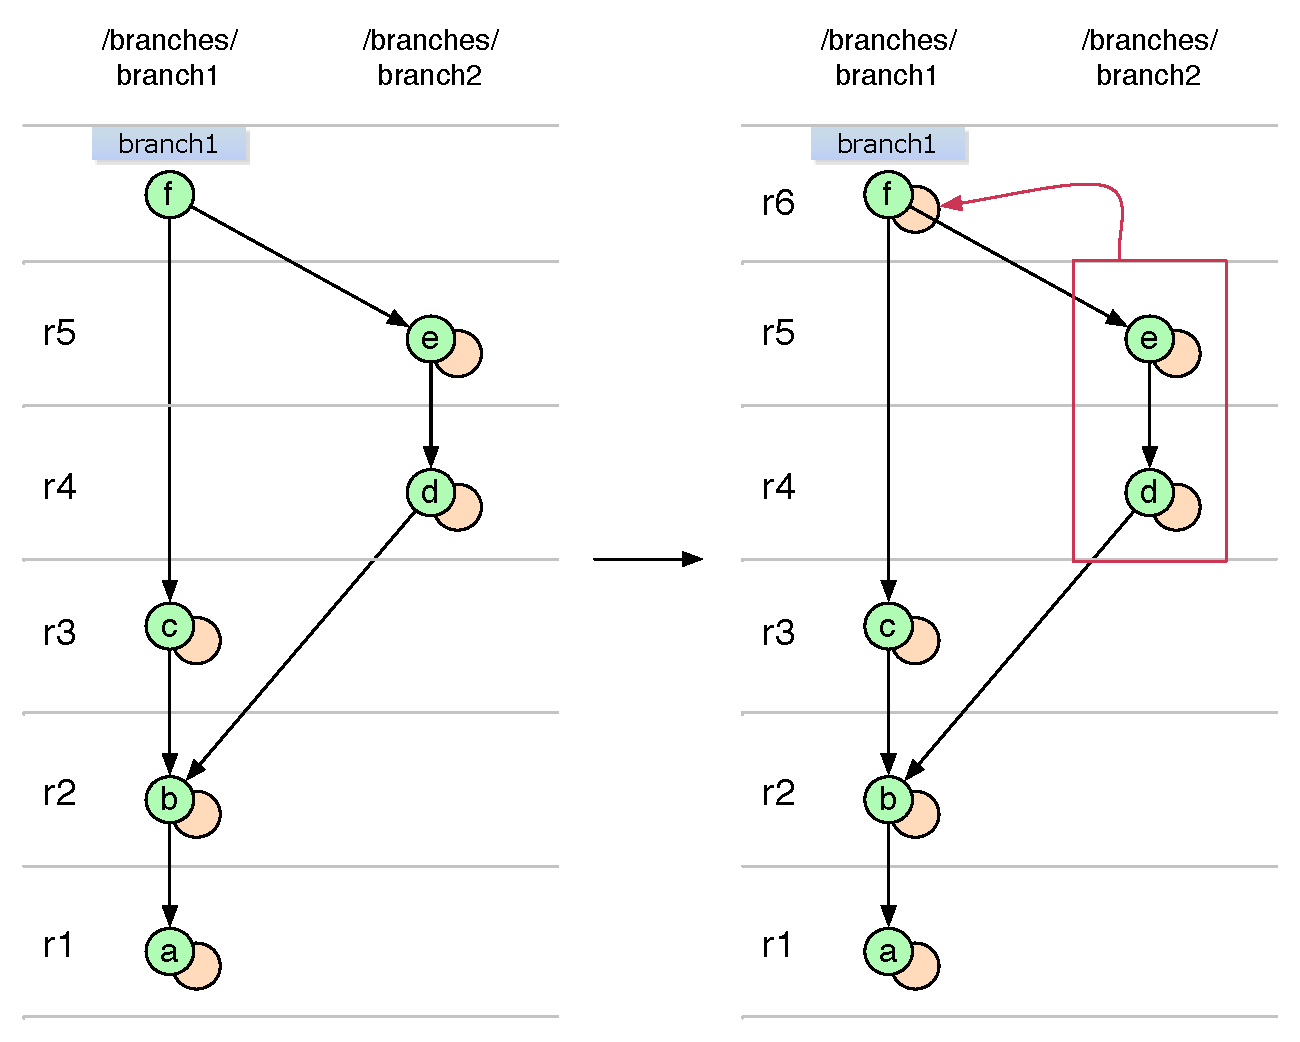
\includegraphics[width=\textwidth]{img/diagrams/simple_merge_git_to_svn.pdf}%
\captionof{figure}{Git merge commit being translated to the change of svn:mergeinfo property.}
\label{simple_merge_git_to_svn}%
\end{center}

Revision \emph{6} is created as a result of commit \emph{f} translation. Then svn:mergeinfo property is updated on /branches/branch1 directory
(red arrow) to reflect merge of commits \emph{d} and \emph{e} made on /branches/branch2 into /branches/branch1. In this 
particular example svn:mergeinfo on /branches/branch1 will be set to "/branches/branch2:4-5" value.
\\\\
Only commits made on the source (ancestor) branches are included into Subversion svn:mergeinfo, references to the commits on the same branch
are excluded. For instance, in the example above, svn:mergeinfo will not contain "/branches/branch1:1-2". Thus, translation of the merge commit with no common history will result in the same svn:mergeinfo being set in Subversion repository (see diagram \ref{simple_merge_branch_no_parent_git_to_svn})

\begin{center}
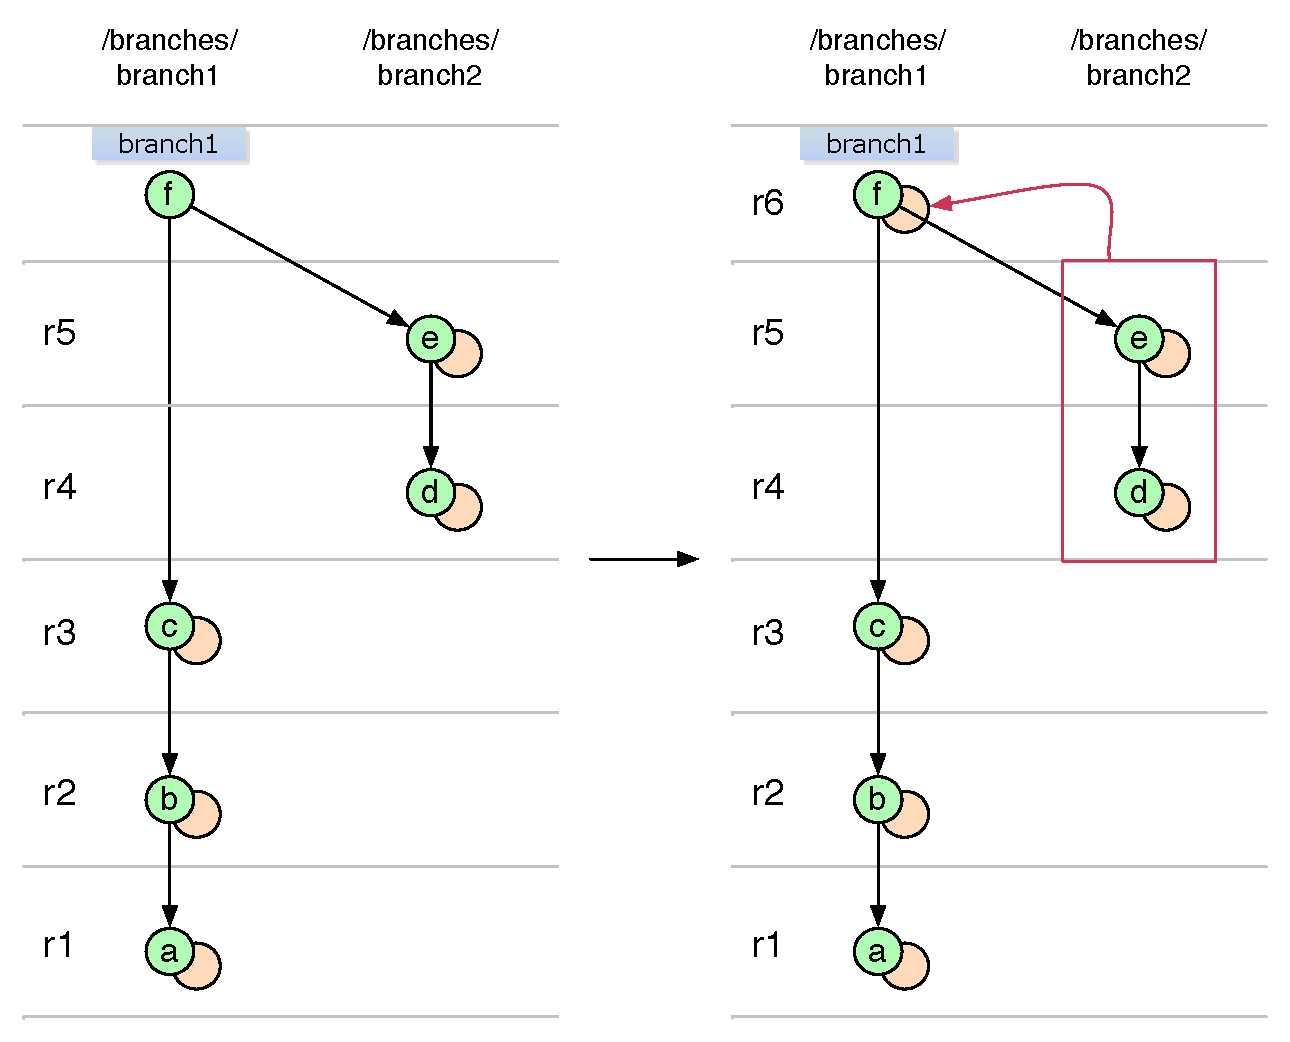
\includegraphics[width=\textwidth]{img/diagrams/simple_merge_branch_no_parent_git_to_svn.pdf}%
\captionof{figure}{Git merge commit being translated to the change of svn:mergeinfo property.}
\label{simple_merge_branch_no_parent_git_to_svn}%
\end{center}

\subsubsection{Translation of Subversion Merges}
\label{section_subversion_merge_to_git}
Merge in Subversion is represented by a revision which includes modification of an svn:mergeinfo property
on a merge target branch directory.
\\\\
Just as translation of the Git merge commit into Subversion revision, 
translation in the opposite direction is performed in two steps:
\begin{itemize}
\item Git commit corresponding to the Subversion revision being translated is created accordingly 
to the rules described in the section \ref{section_revisions_and_commits}.
\item Additional parent commits are set on the Git commit just created. 
Whether and what parent commits are added, depends on the svn:mergeinfo property value.
\end{itemize}
To translate svn:mergeinfo property value into a set of parent commits the following algorithm is used:
\begin{enumerate}
\item For each revision range defined by svn:mergeinfo, Git commit corresponding to the first range
revision is located.
\item For each located Git commit its parents are traversed until merge-base commit or commit without
parent is encountered. All traversed Git commits are added to the merge path.
\item Each computed merge path is translated into revision range. In case this range is present in 
svn:mergeinfo, first path commit is added as a parent to the set of parent commits.
\end{enumerate}
Diagrams \ref{simple_merge_svn_to_git} and \ref{simple_merge_branch_no_parent_svn_to_git} provides
examples of svn:mergeinfo property (shown as a red arrow) change translation into Git Merge commit (commit \emph{f} on both
diagrams).

\begin{center}
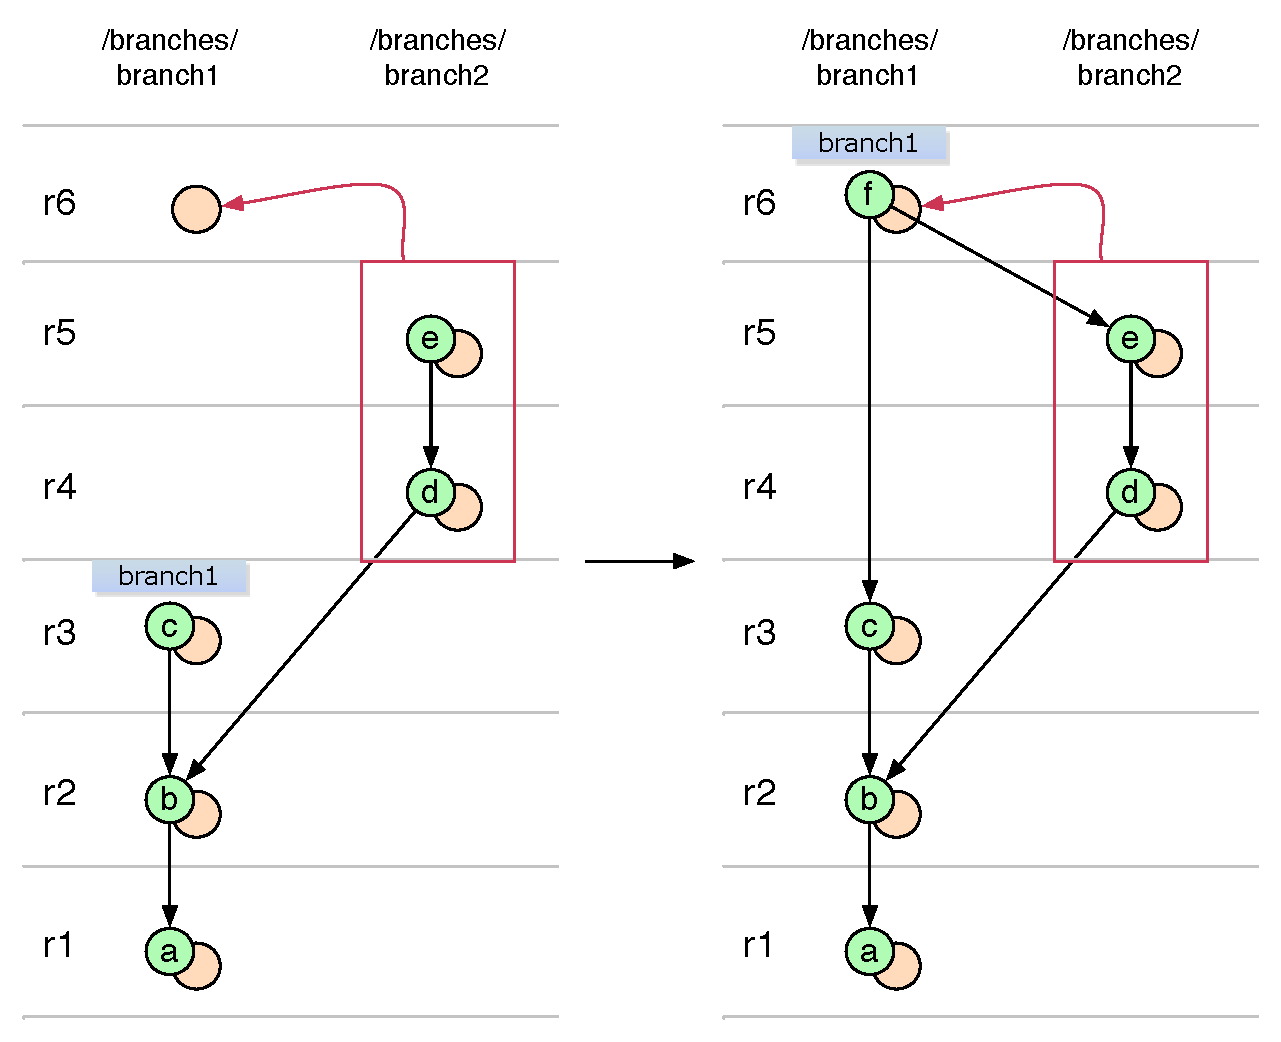
\includegraphics[width=\textwidth]{img/diagrams/simple_merge_svn_to_git.pdf}%
\captionof{figure}{svn:mergeinfo property change being translated into merge commit creation.}
\label{simple_merge_svn_to_git}%
\end{center}

\begin{center}
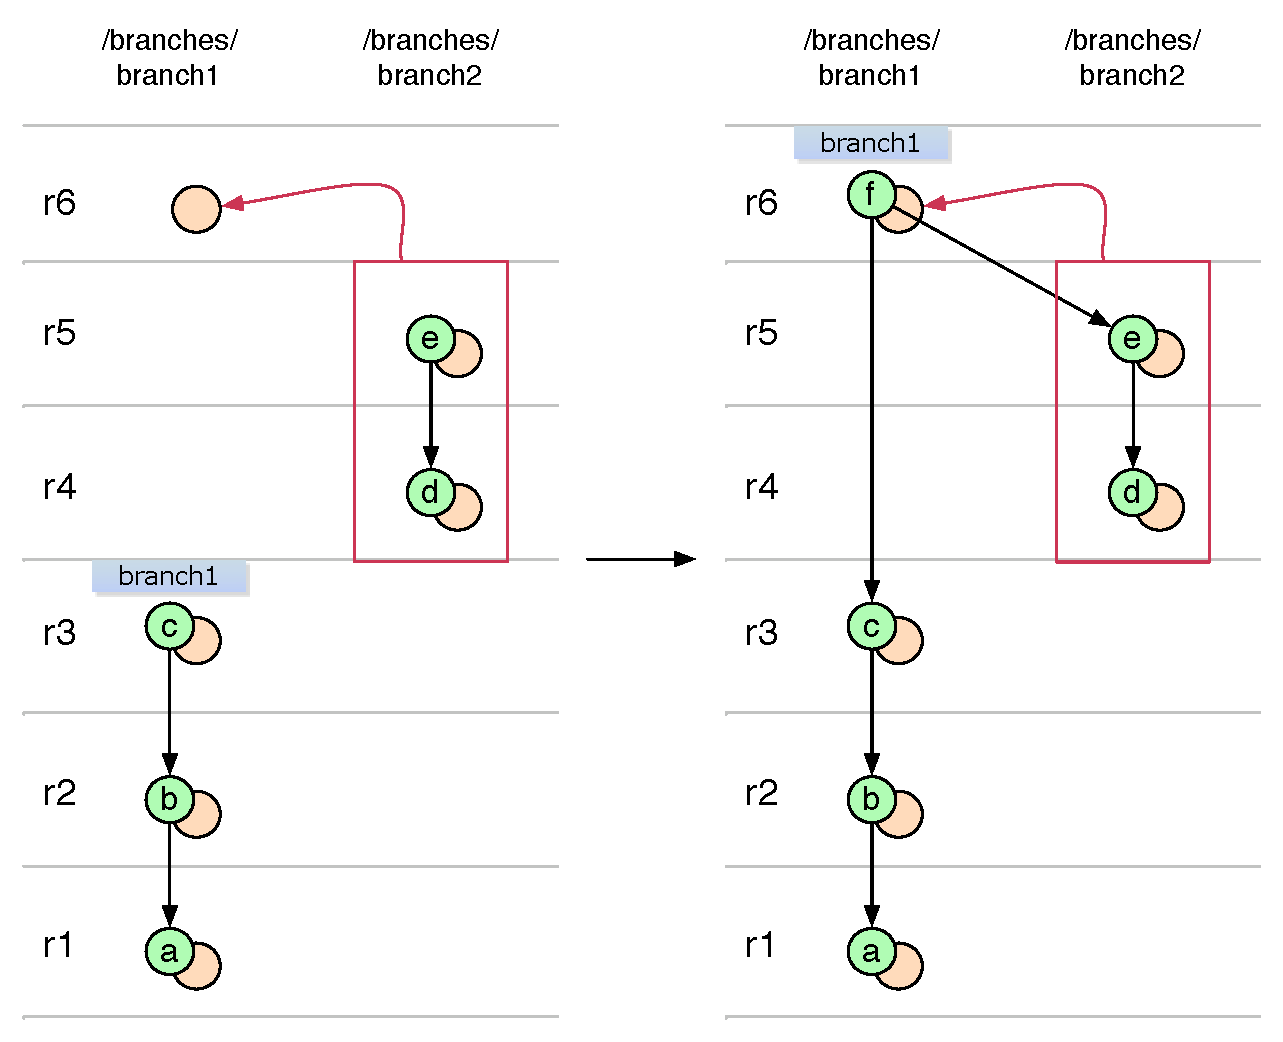
\includegraphics[width=\textwidth]{img/diagrams/simple_merge_branch_no_parent_svn_to_git.pdf}%
\captionof{figure}{svn:mergeinfo property change being translated into merge commit creation.}
\label{simple_merge_branch_no_parent_svn_to_git}%
\end{center}

\subsubsection{Subversion Cherry-Pick Merges}

Subversion tracks merges of the individual revisions, a feature also known as cherry-pick merges. 
Git is able to perform cherry-pick merges but it has no means to track these merges as part of merge commit history. 
Hence, changes of the svn:mergeinfo Subversion property that result from the cherry-pick merge (i.e. changes that add individual revisions to the svn:mergeinfo) are
translated into the regular Git commit with a single parent commit (see diagram \ref{no_merge_commit_on_cherry_pick_svn_to_git}).
\begin{center}
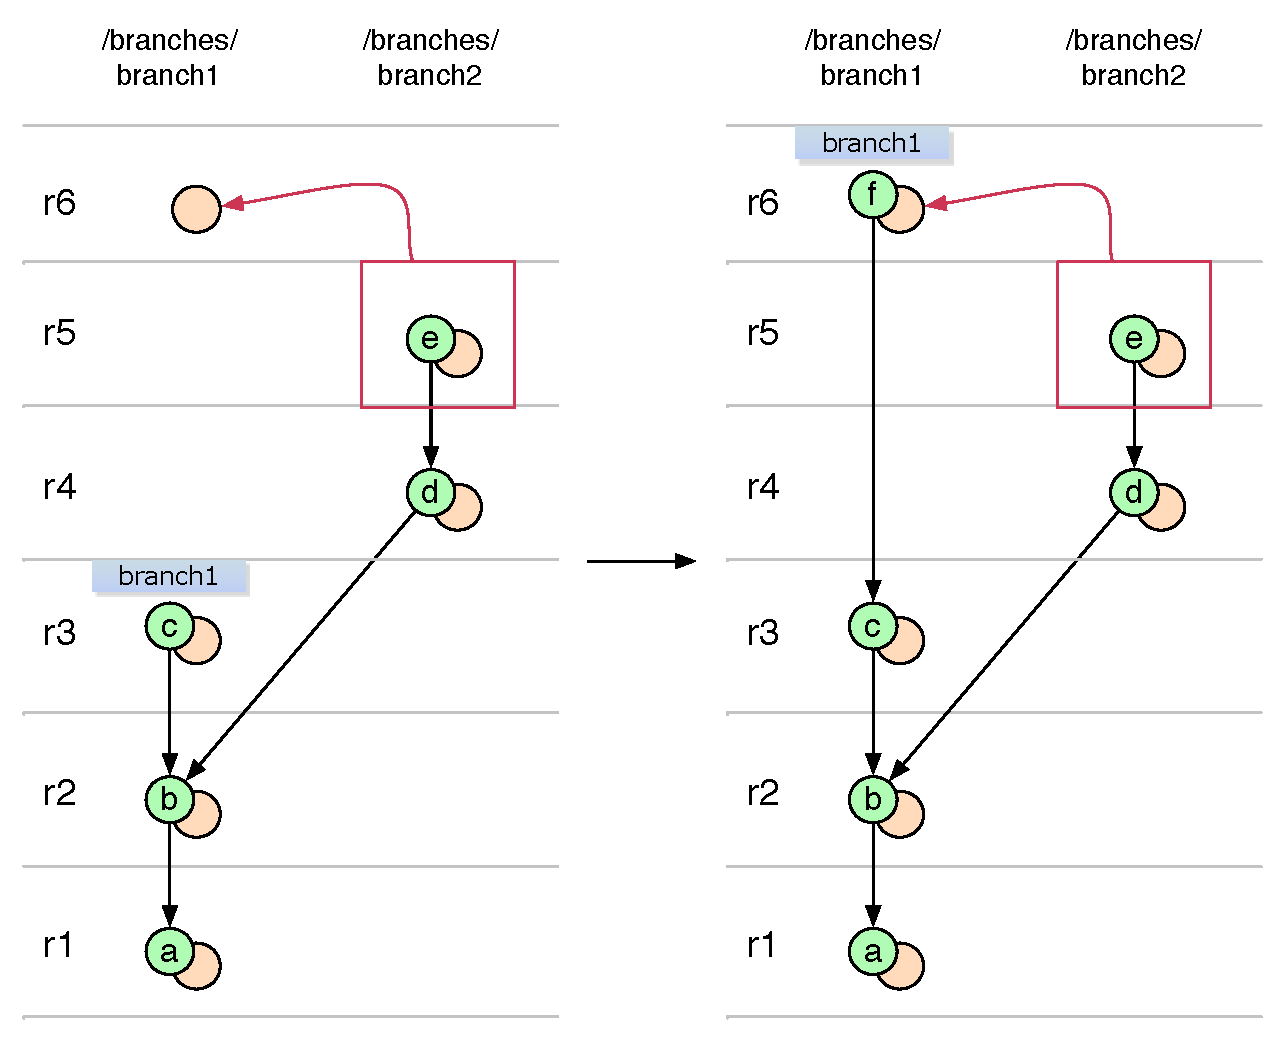
\includegraphics[width=\textwidth]{img/diagrams/no_merge_commit_on_cherry_pick_svn_to_git.pdf}%
\captionof{figure}{Cherry-pick merge being translated to ordinary commit.}
\label{no_merge_commit_on_cherry_pick_svn_to_git}%
\end{center}

Eventually, a sequence of cherry-pick merges may result in svn:mergeinfo property value which could 
be translated to the set of parent commits (see translation algorithm in the section \ref{section_subversion_merge_to_git}).
In that case last modification of the svn:mergeinfo property is translated into a Git merge commit, as 
shown on the diagrams \ref{merge_commit_on_double_cherry_pick_svn_to_git} and \ref{merge_commit_on_double_cherry_pick_branch_no_parent_svn_to_git},
where Git commit \emph{g} is a Git merge commit.

\begin{center}
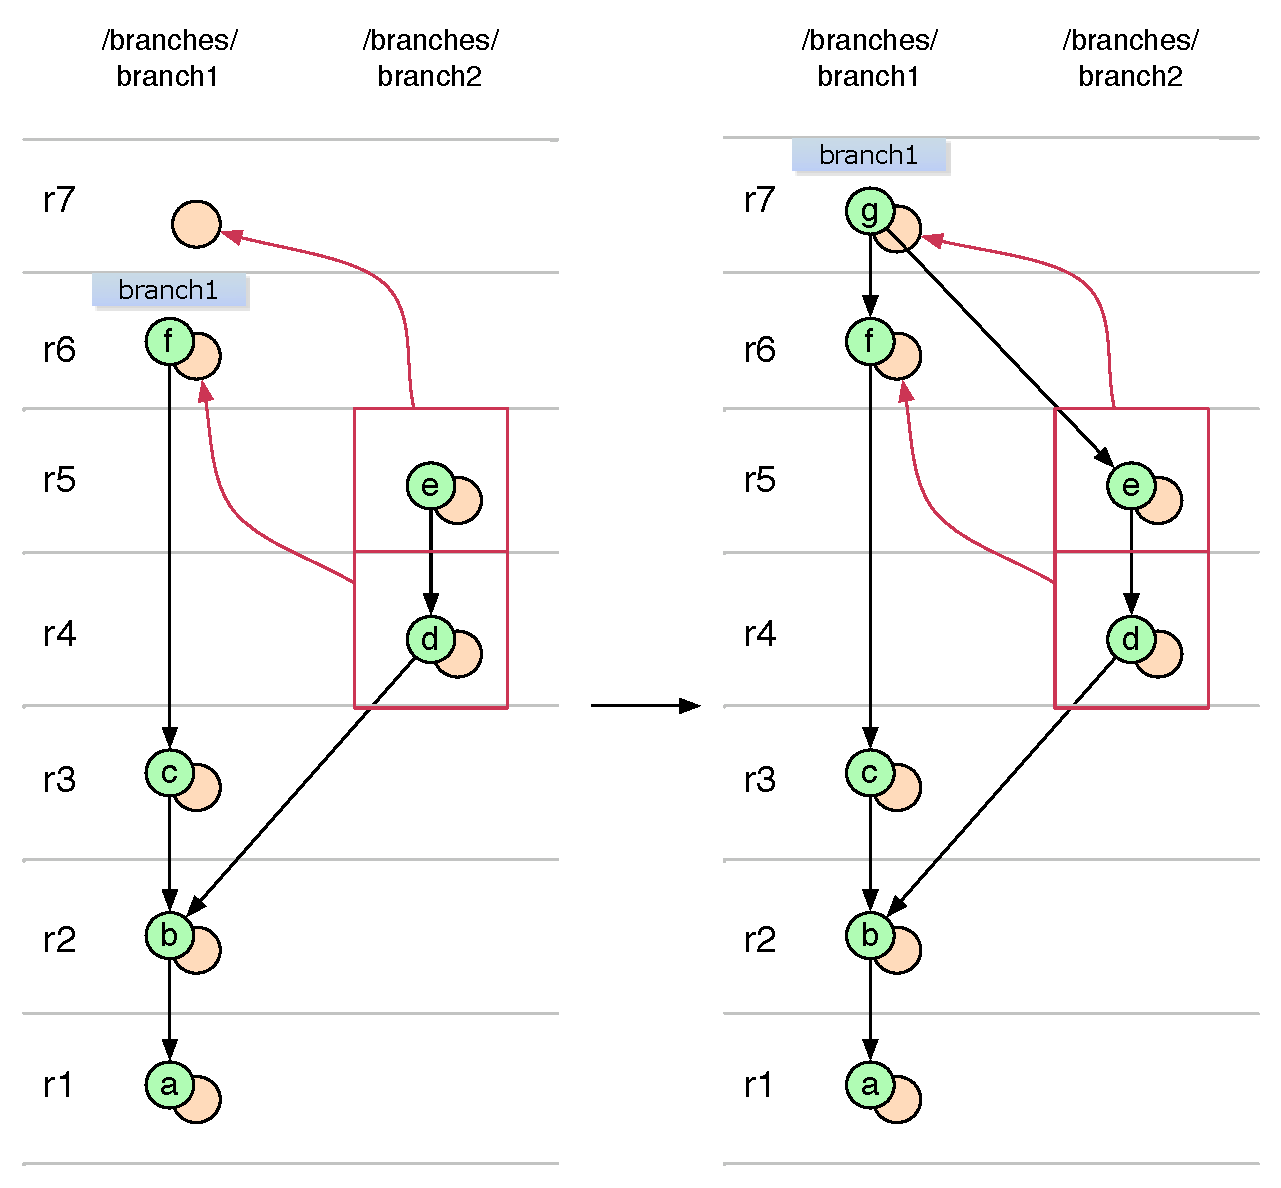
\includegraphics[width=\textwidth]{img/diagrams/merge_commit_on_double_cherry_pick_svn_to_git.pdf}%
\captionof{figure}{A sequence of cherry-pick merges being translated to merge commit.}
\label{merge_commit_on_double_cherry_pick_svn_to_git}%
\end{center}

\begin{center}
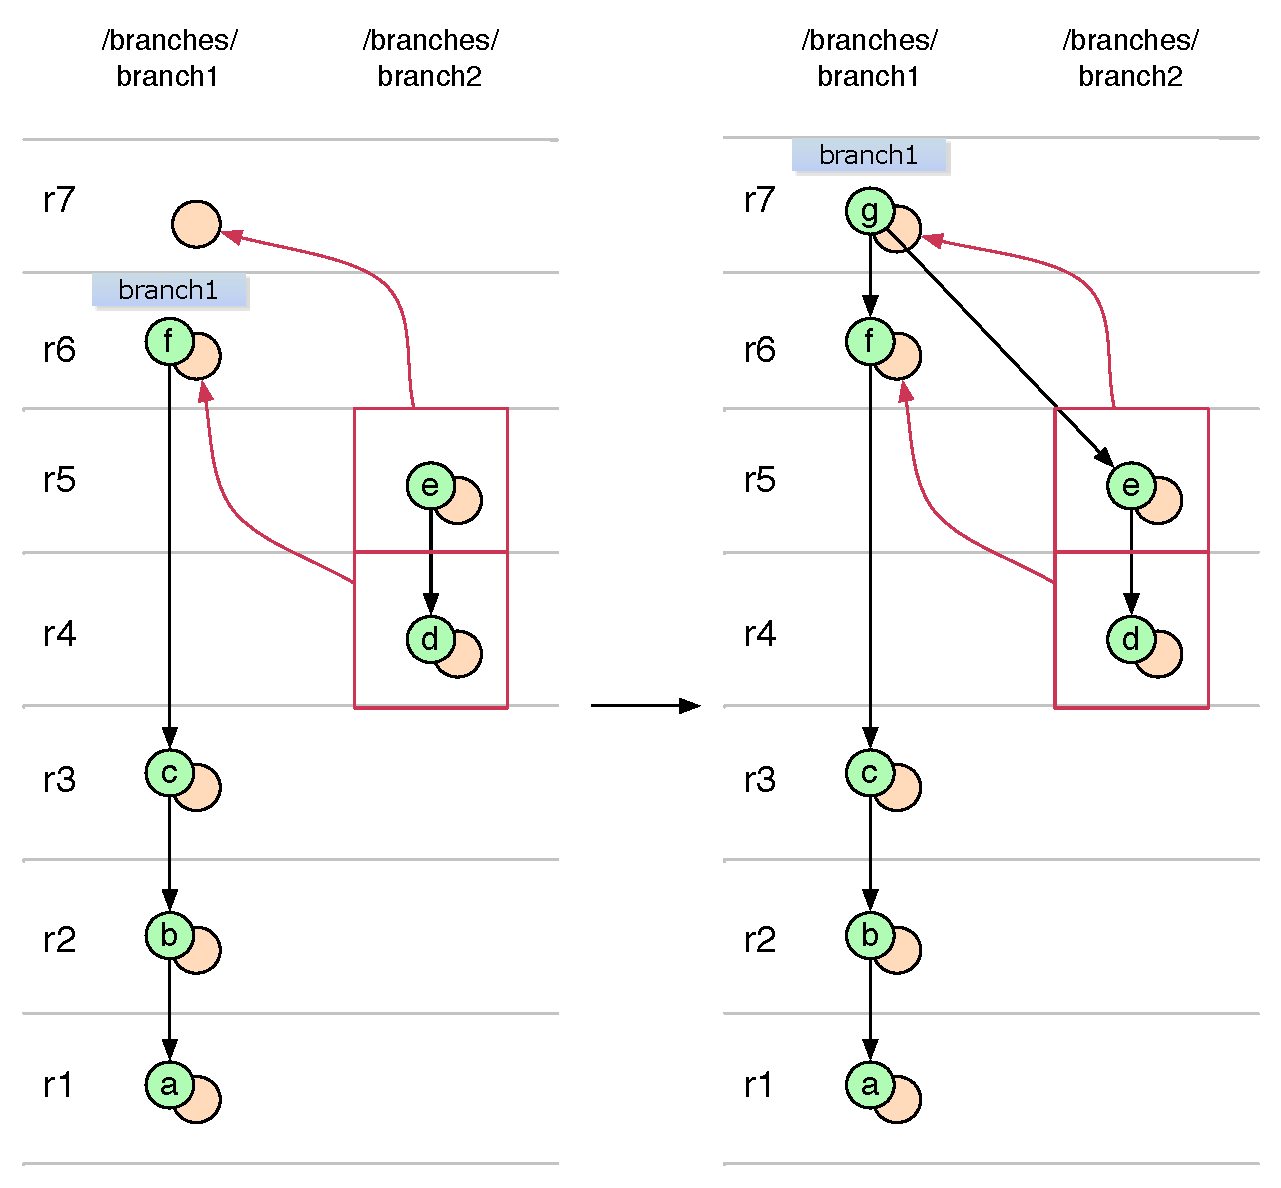
\includegraphics[width=\textwidth]{img/diagrams/merge_commit_on_double_cherry_pick_branch_no_parent_svn_to_git.pdf}%
\captionof{figure}{A sequence of cherry-pick merges being translated to merge commit.}
\label{merge_commit_on_double_cherry_pick_branch_no_parent_svn_to_git}%
\end{center}

\subsubsection{Shelf Branches}
\label{shelf_branches}

Git user is able to push an arbitrary number of commits at once. This set of Git commits might include Git merge commit, 
so that some of the Git commits in the set are arranged into the structure we call \emph{shelf}. In general, \emph{shelf}
translation includes:
\begin{itemize}
\item Creation of a Subversion branch which correspond to the \emph{shelf};
\item Translation of the \emph{shelved} commits into revisions on that \emph{shelf} branch;
\item Translation of the merge commit into revision on the main branch, with svn:mergeinfo including all revisions
of the \emph{shelf} branch.
\end{itemize}
Examples of \emph{shelf} translation are shown in the diagrams \ref{boat_merge_named_shelve_git_to_svn} and \ref{boat_merge_shelve_is_normal_branch_git_to_svn}.
In these examples it is possible to determine name for the \emph{shelf} branch either because branch reference points directly to the 
last \emph{shelf} commit (diagram \ref{boat_merge_named_shelve_git_to_svn}) or to the commit which originates from the \emph{shelf} (diagram \ref{boat_merge_shelve_is_normal_branch_git_to_svn}).
\begin{center}
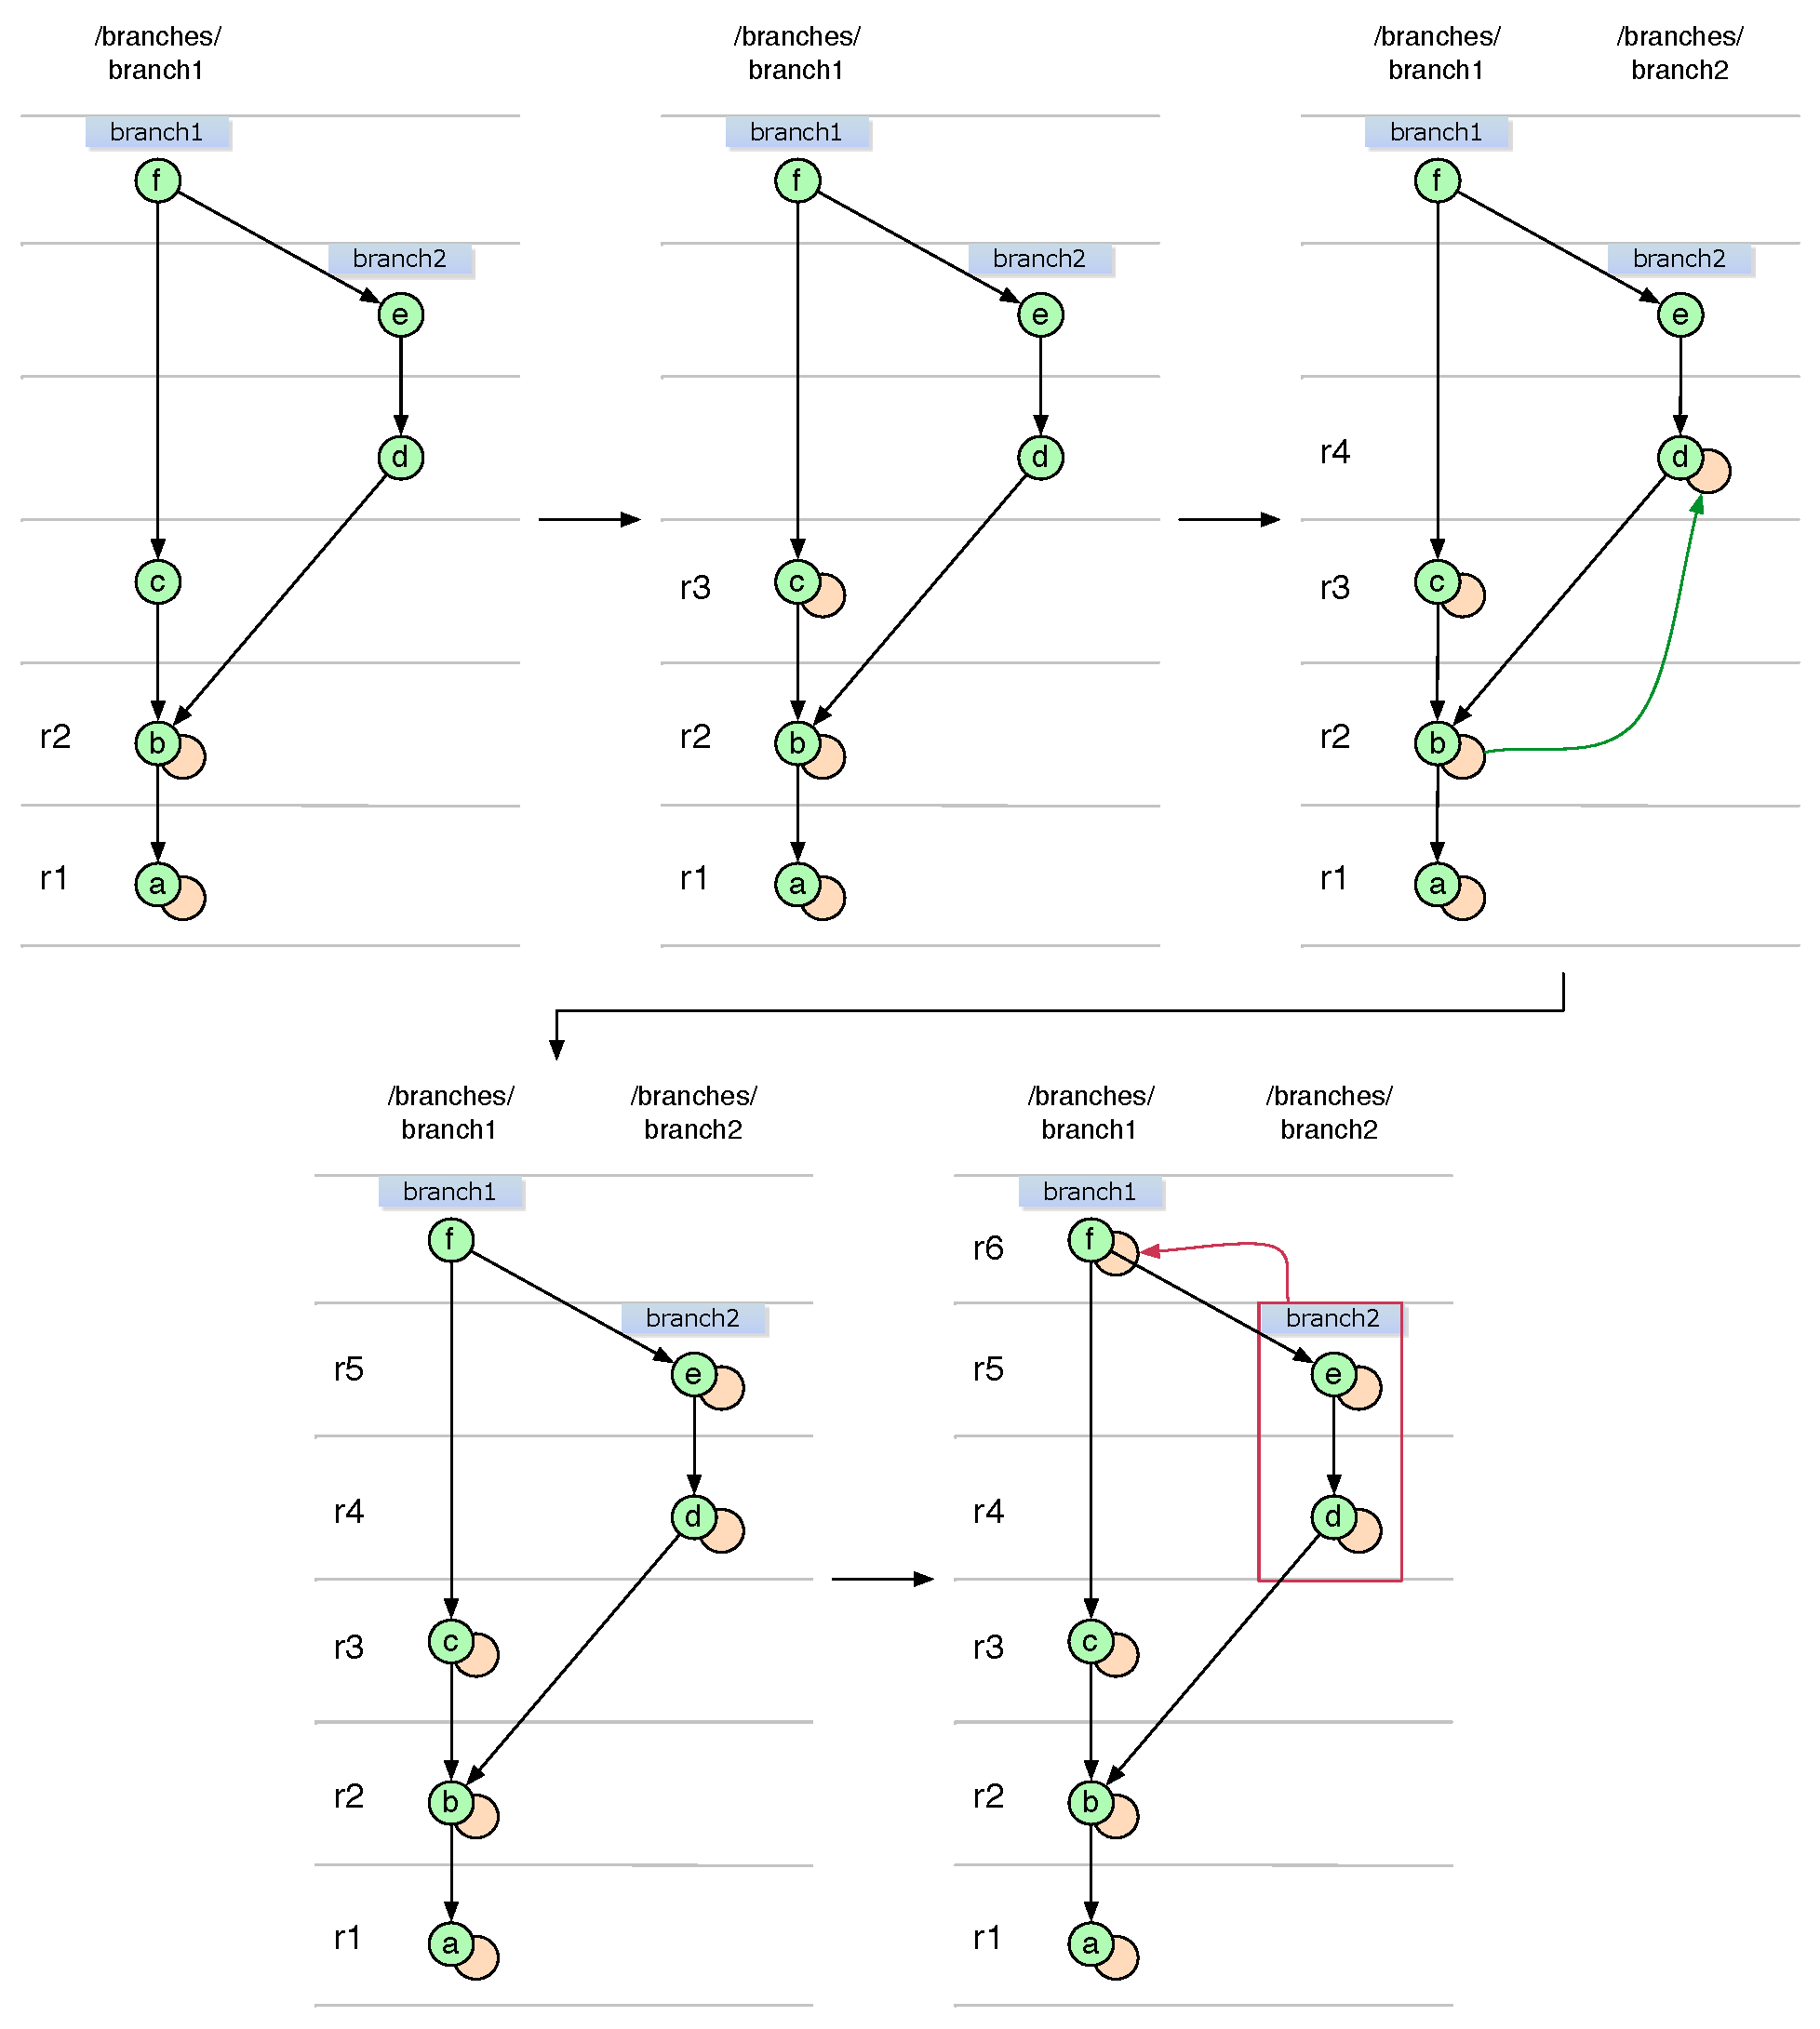
\includegraphics[width=\textwidth]{img/diagrams/boat_merge_named_shelve_git_to_svn.pdf}%
\captionof{figure}{Merge of Git branch which is available from another branch being translated to a sequence of Subversion revisions.}
\label{boat_merge_named_shelve_git_to_svn}%
\end{center}
\begin{center}
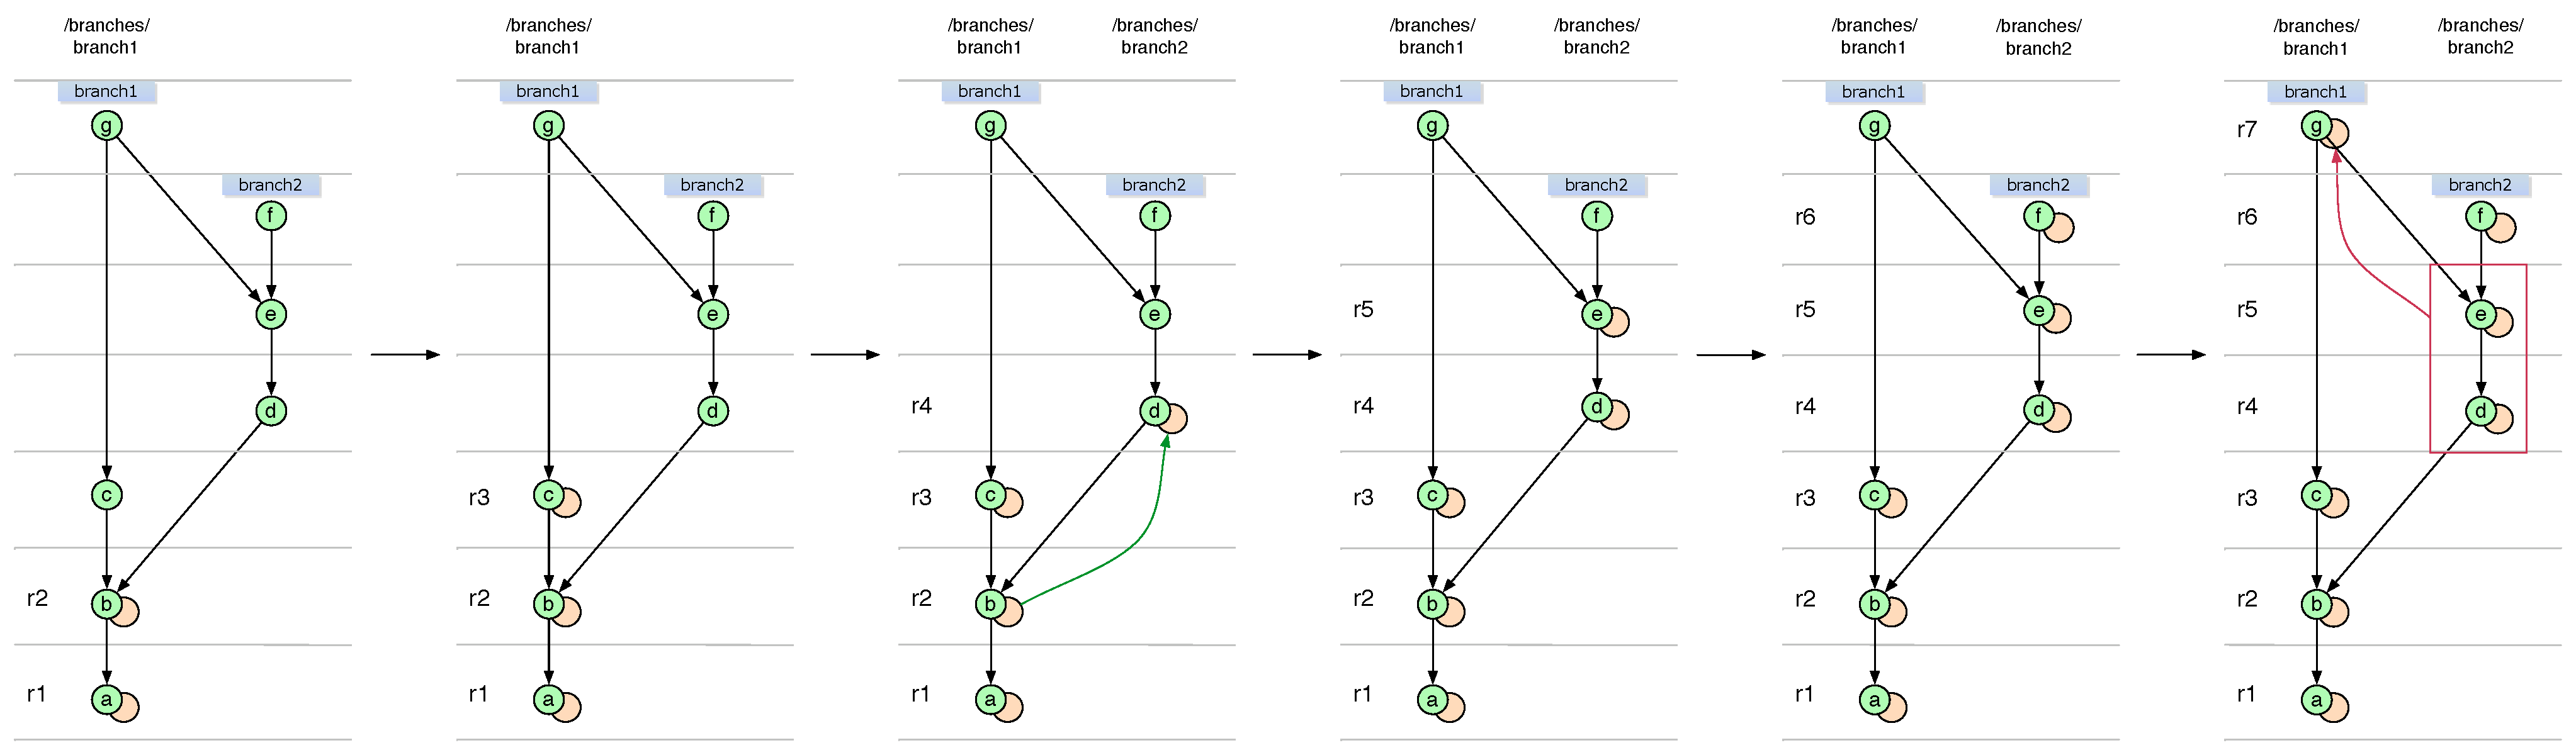
\includegraphics[width=\textwidth]{img/diagrams/boat_merge_shelve_is_normal_branch_git_to_svn.pdf}%
\captionof{figure}{Merge of Git branch which is available from another branch being translated to a sequence of Subversion revisions.}
\label{boat_merge_shelve_is_normal_branch_git_to_svn}%
\end{center}

In certain cases, it is not possible to determine name for the \emph{shelf} branch, as there is no branch reference pointing to
the \emph{shelved} commits. In such case Translator creates temporary branch named after the first shelf commit author and 
deletes this temporary branch in the revision which corresponds to the merge commit (see diagram \ref{boat_merge_git_to_svn}). 
\\\\
To reduce clutter, anonymous temporary branch is created in the /shelves/ top-level Subversion directory, not in the /branches/ one where named branches reside. % and removed as soon as shelf is merged into the certain branch.

\begin{center}
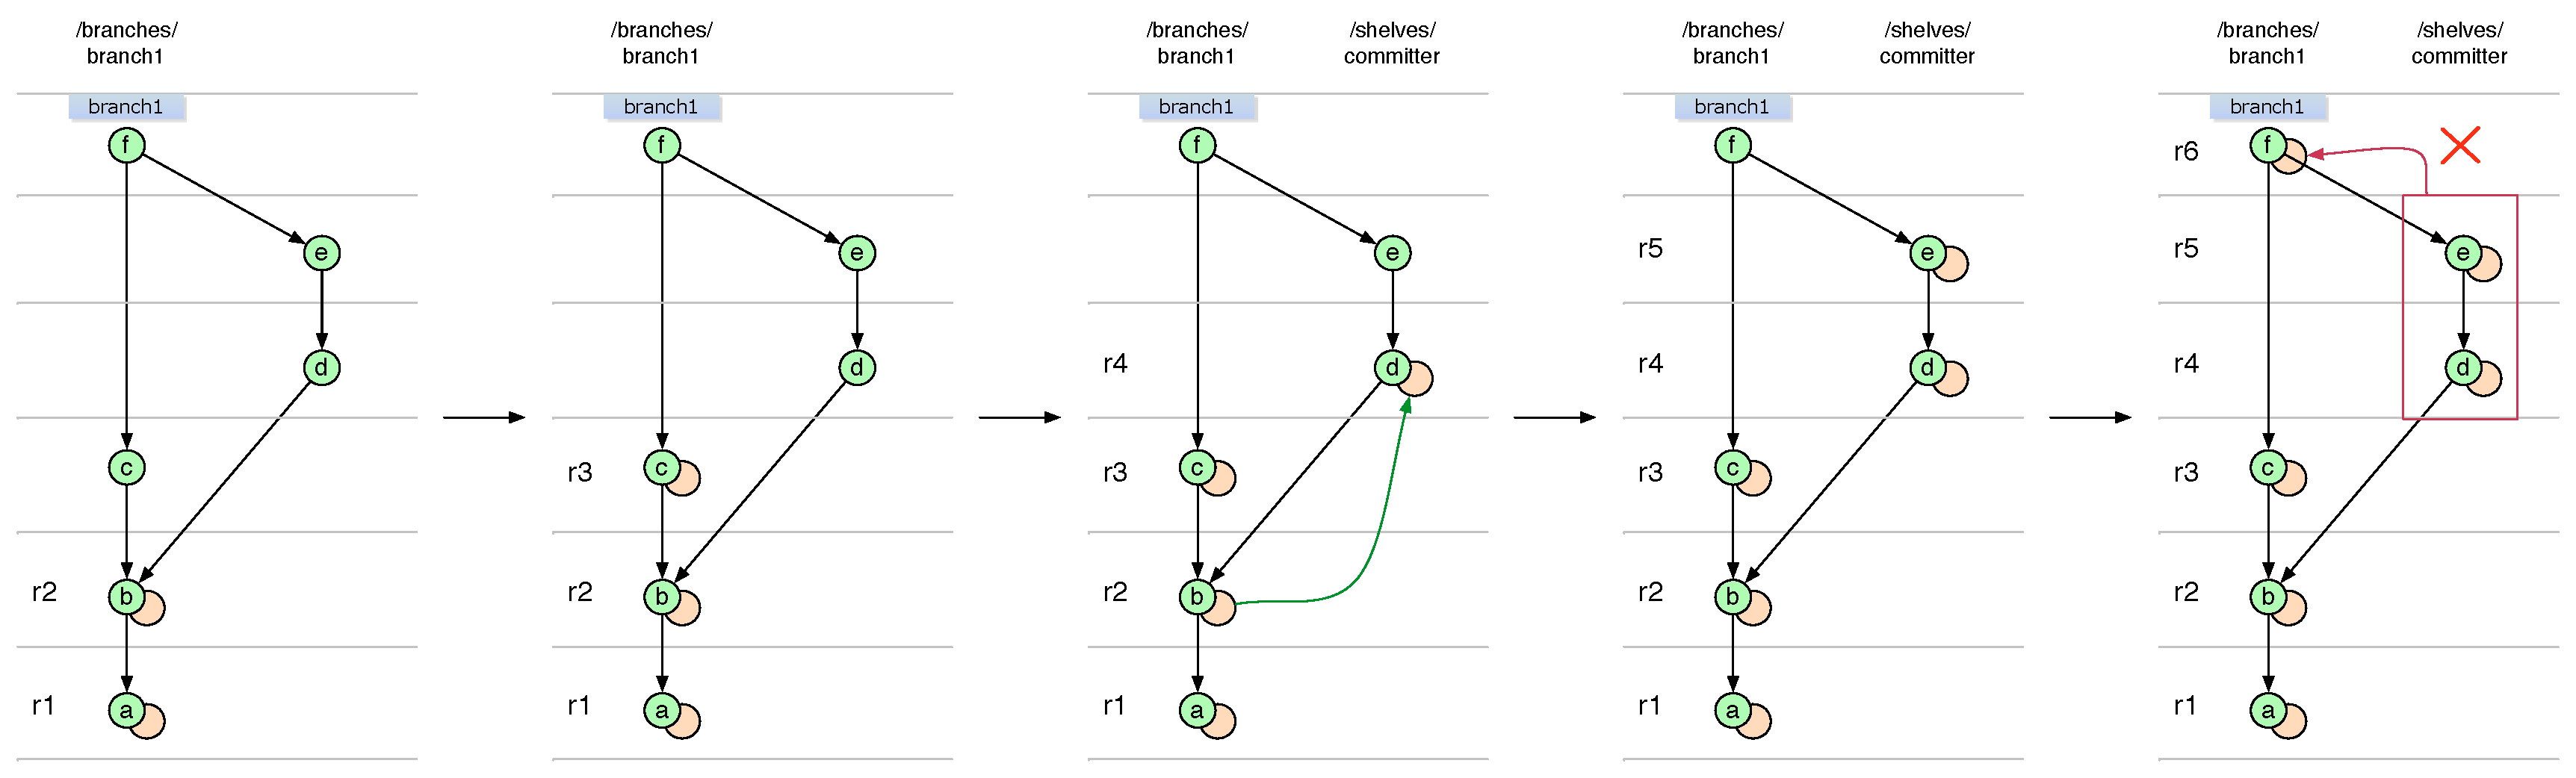
\includegraphics[width=\textwidth]{img/diagrams/boat_merge_git_to_svn.pdf}%
\captionof{figure}{Merge of anonymous Git branch being translated to a sequence of Subversion revisions.}
\label{boat_merge_git_to_svn}%
\end{center}
\newpage
\subsubsection{Complex Merge History}

On Git merge commits translation, Translator might encounter Git merge commit which refer to the parent commit, which,
in its turn, refers to another merge commit.
\\\\
Subversion svn:mergeinfo property which have to be translated to a Git merge commit, might refer to the multiple branches,
either directly enumerating all branches and revisions, or indirectly, by referring to the branch which has svn:mergeinfo property set on it referring to another branch.
\\\\
Below are examples of the \emph{complex merges}. On translating of such merges, Translator takes into account both
directly and indirectly referenced changes and performs translation accordingly to the composite set of the 
changes referenced by the merge commits or by the svn:mergeinfo properties.
\\\\
Shown below are examples of the complex merge history translation.
\\\\
The first use case is depicted at diagram \ref{nested_merge_full_mergeinfo_git_to_svn}. 
Commit \emph{i} is the merge commit of branches branch3 and branch1. 
But branch1 has a commit \emph{f} which is commit merged branch2 into branch1. 
For that case at corresponding revision r9 we add svn:mergeinfo property to branch3 which includes the merge history of all commits being merged at commit \emph{i}.

\begin{center}
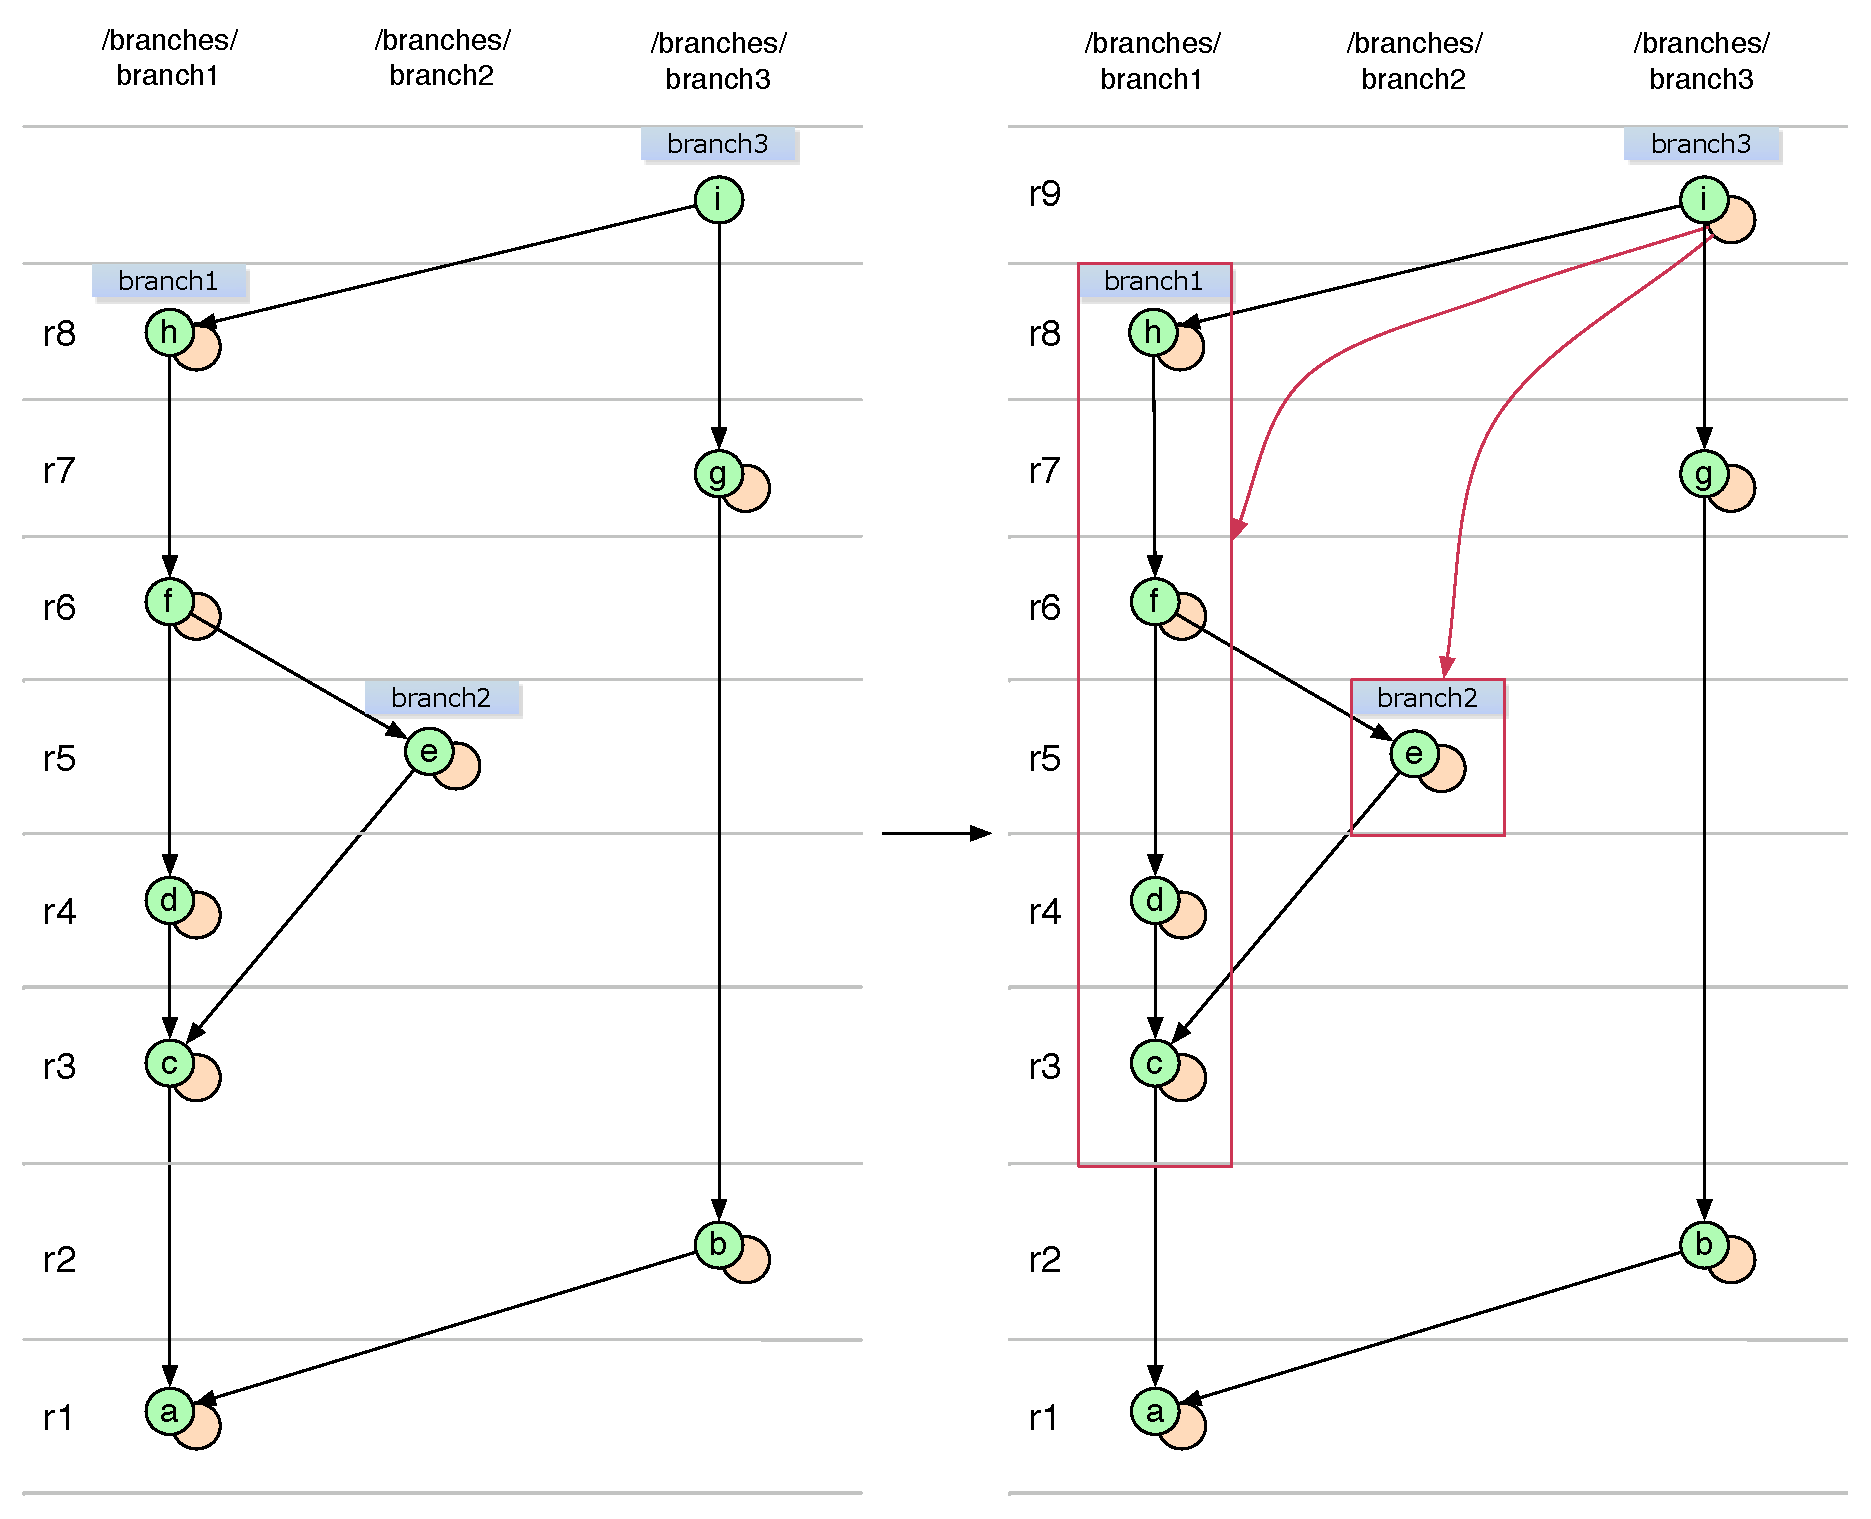
\includegraphics[width=\textwidth]{img/diagrams/nested_merge_full_mergeinfo_git_to_svn.pdf}%
\captionof{figure}{Merge of Git branch which is available from another branch being translated to a sequence of Subversion revisions.}
\label{nested_merge_full_mergeinfo_git_to_svn}%
\end{center}

The mirror of this use case is depicted at diagram \ref{nested_merge_full_mergeinfo_svn_to_git}. Subversion user merged all the revision which represent the whole history of Git commits being merged at commit \emph{i}.

\begin{center}
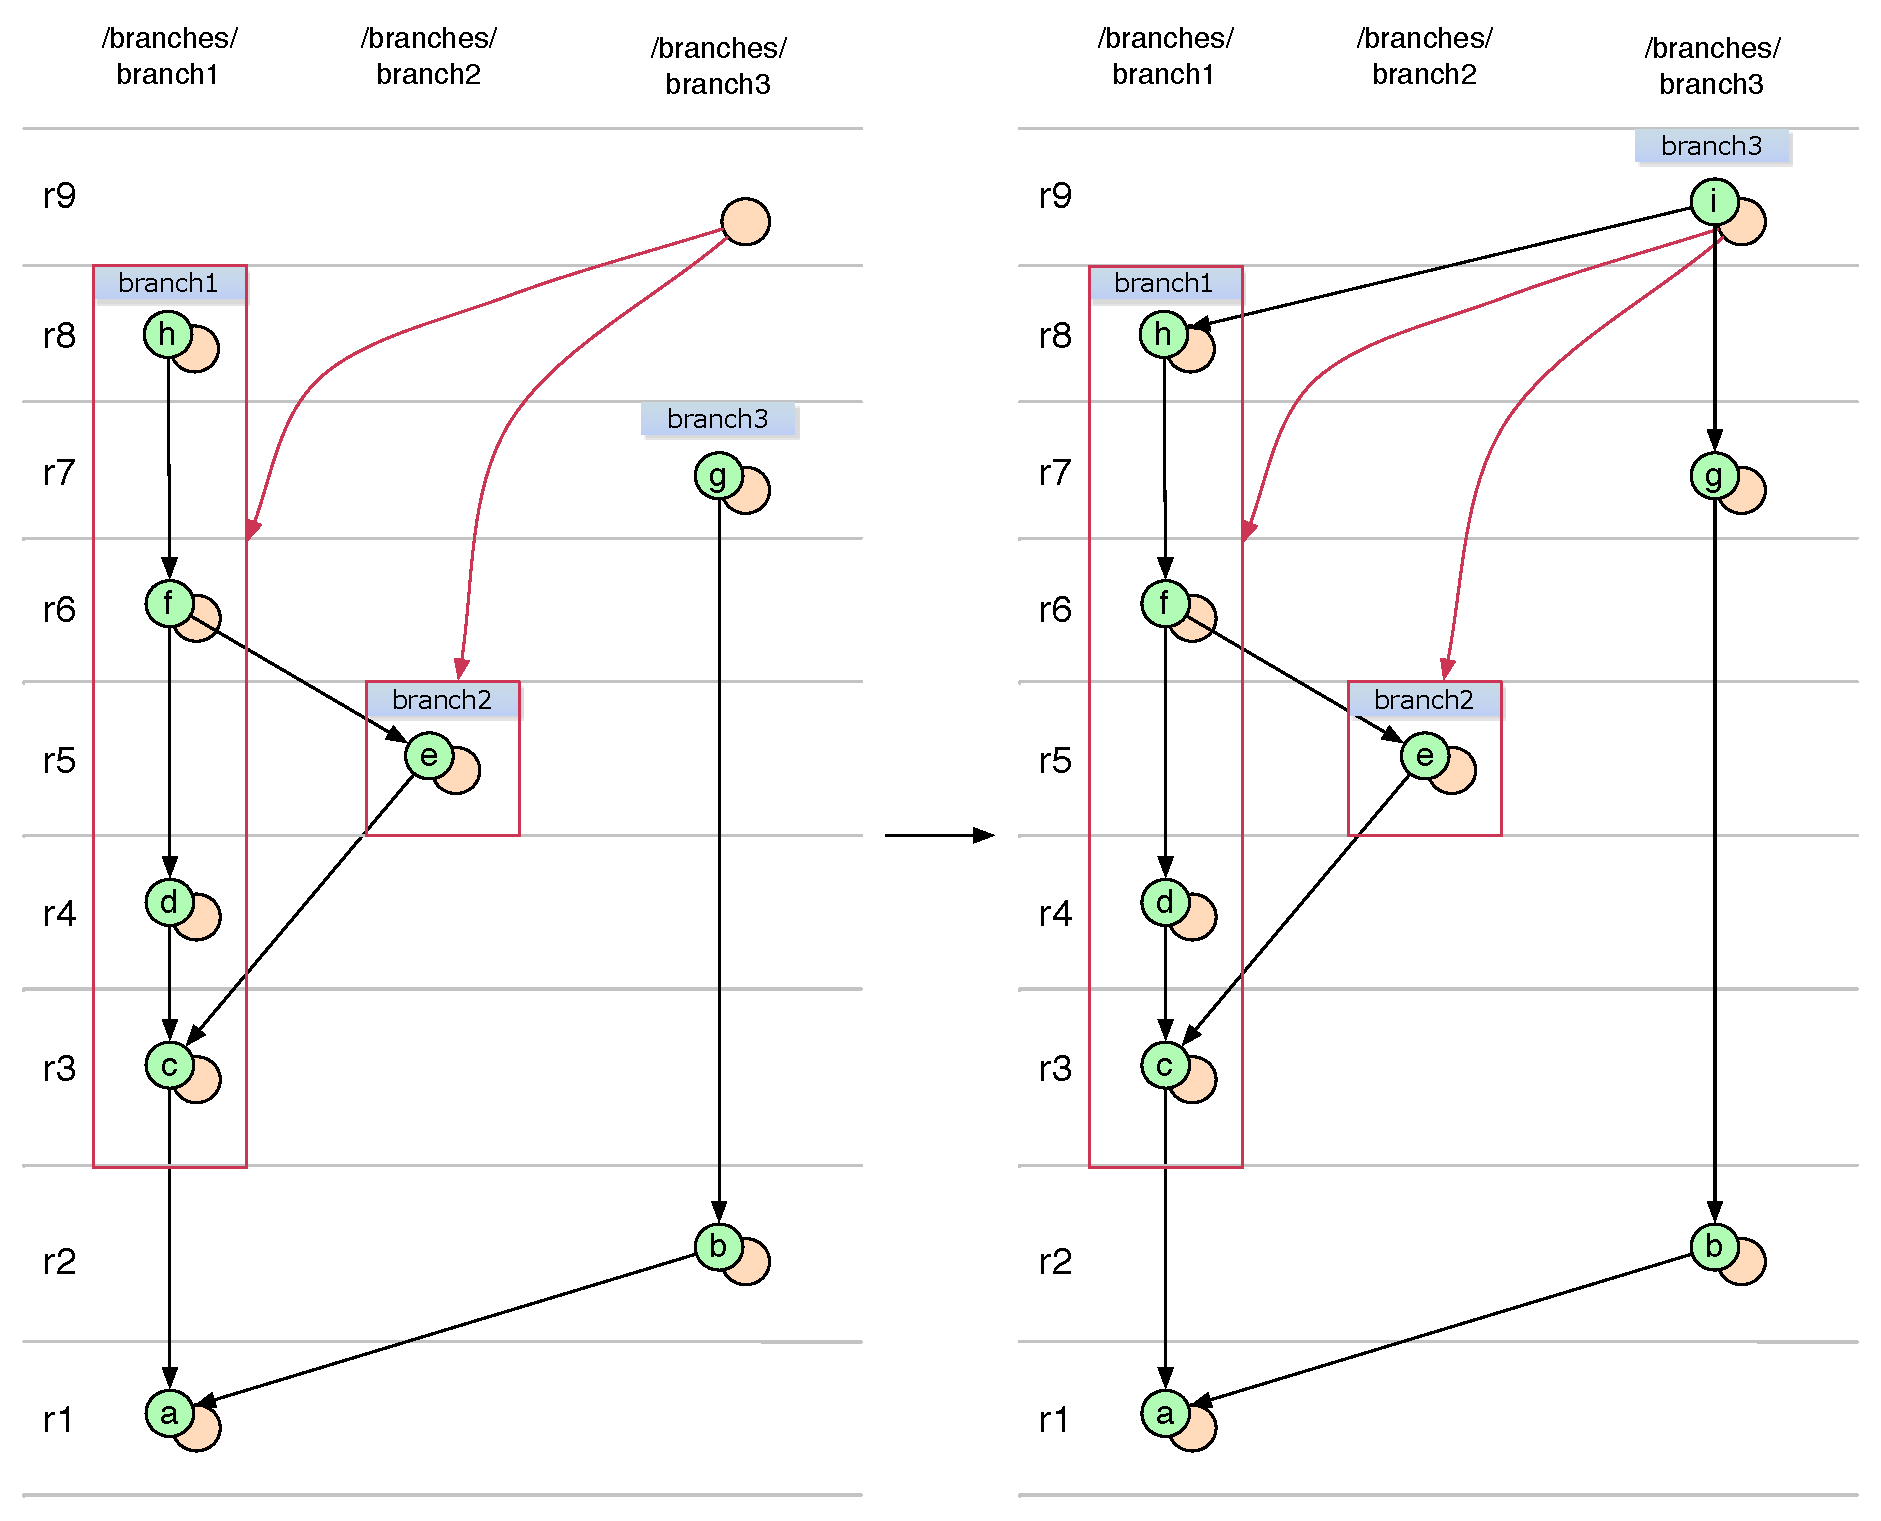
\includegraphics[width=\textwidth]{img/diagrams/nested_merge_full_mergeinfo_svn_to_git.pdf}%
\captionof{figure}{Merge of Git branch which is available from another branch being translated to a sequence of Subversion revisions.}
\label{nested_merge_full_mergeinfo_svn_to_git}%
\end{center}

Slightly modified scenario is depicted at diagram \ref{nested_merge_partly_mergeinfo_svn_to_git}. Subversion user didn't include /branches/branch2@r5 into merge history explicitly. But this change is already included via revision /branches/branch1@r6, thus commit \emph{e} is included into merge history of revision r9 implicitly. As result Translator is able to create commit \emph{i} corresponding to revision r9 and set two parents to it.

\begin{center}
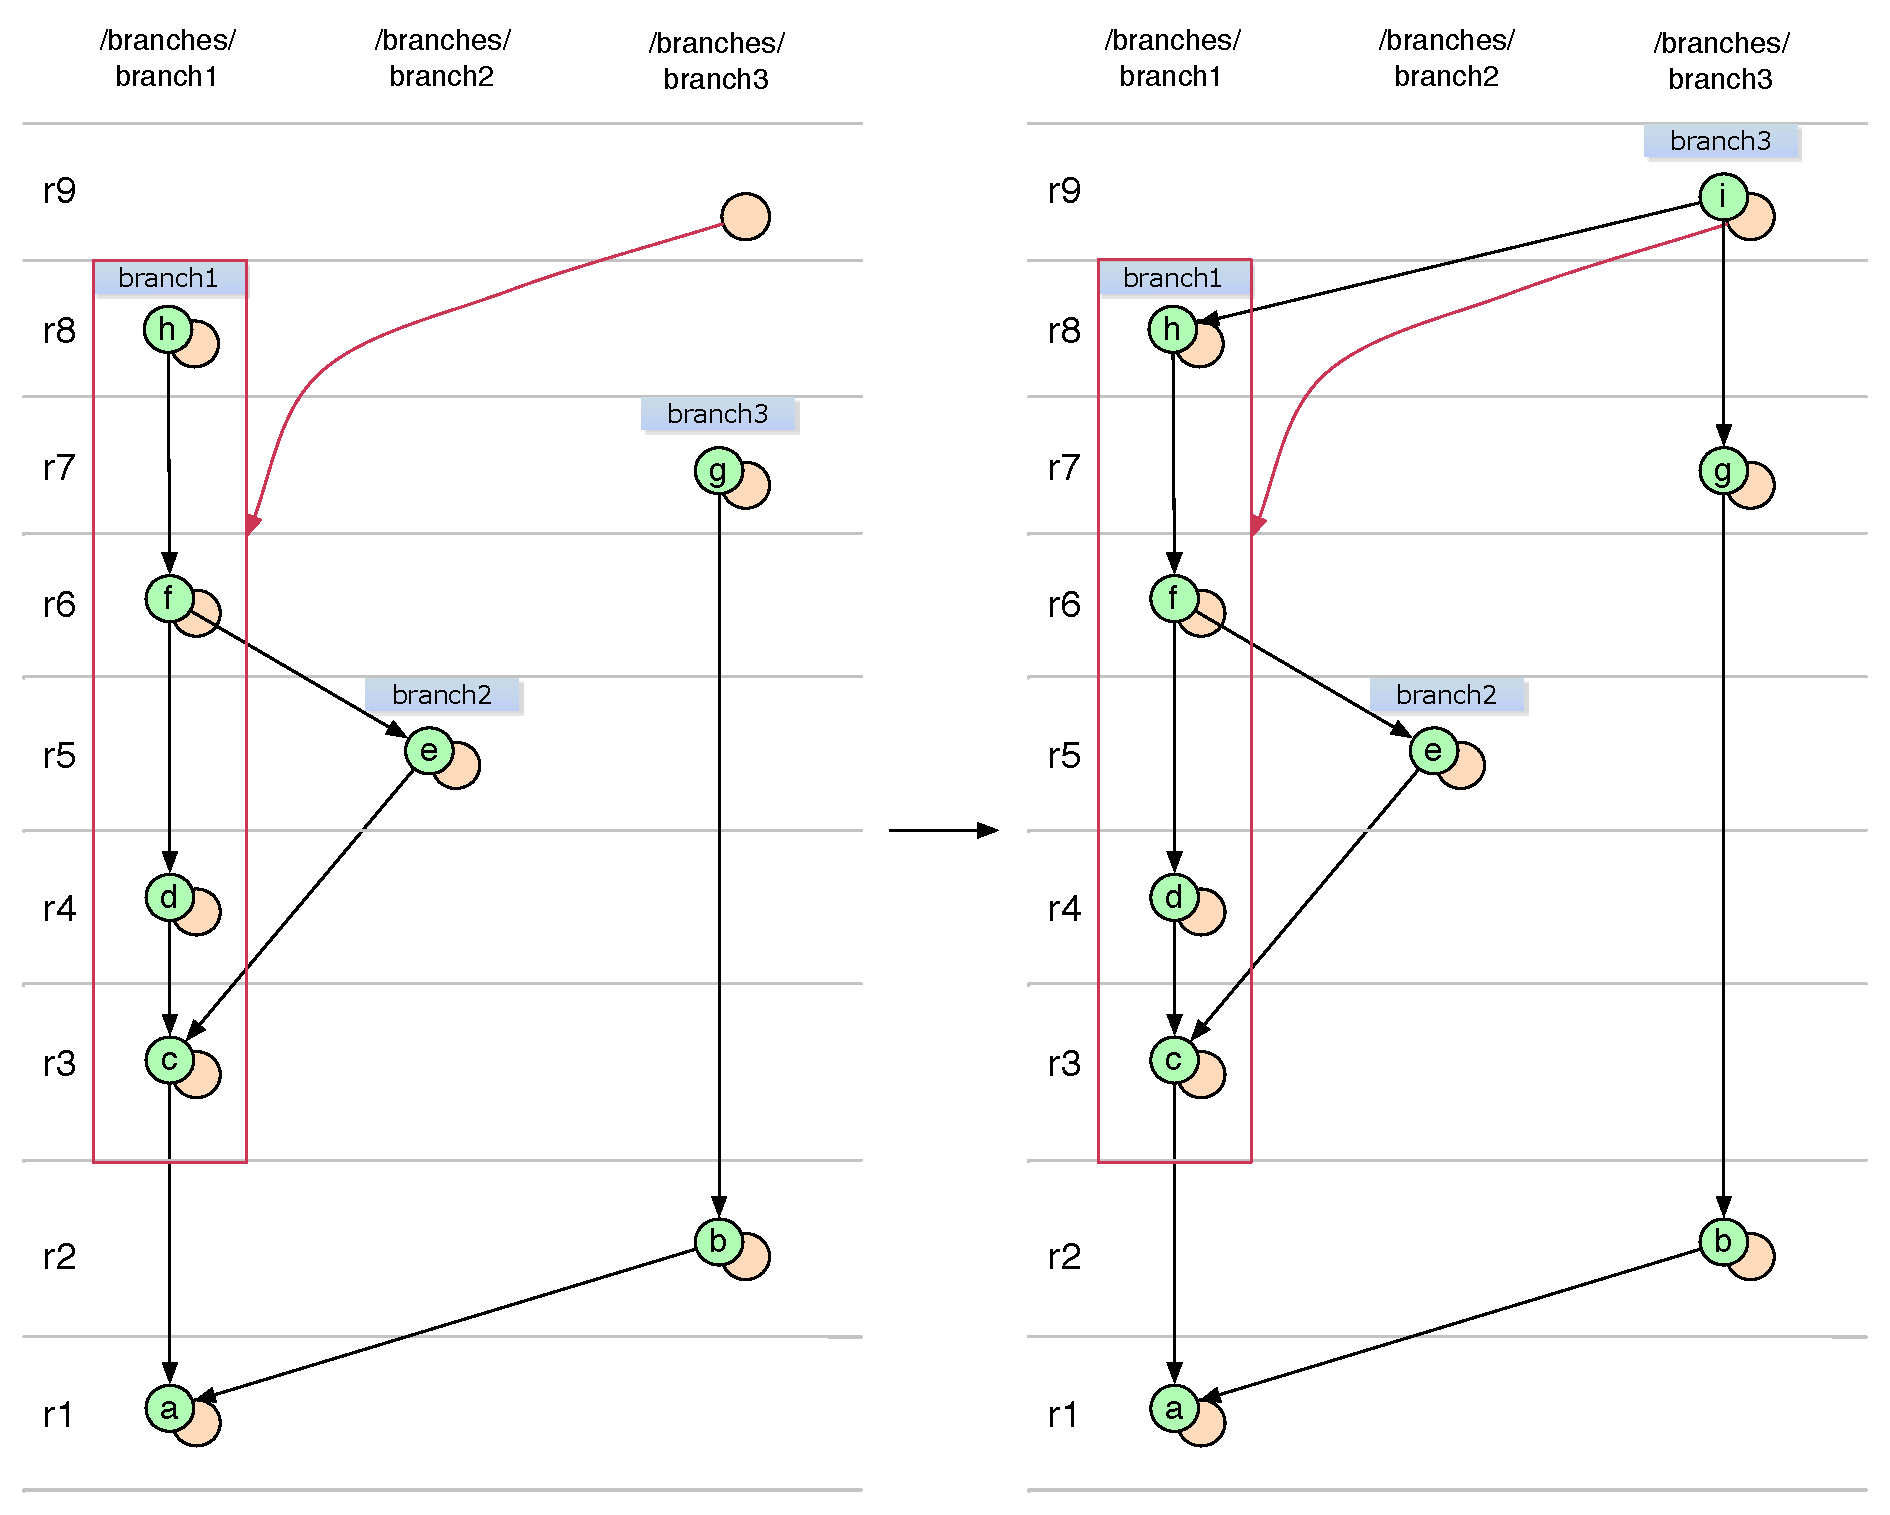
\includegraphics[width=\textwidth]{img/diagrams/nested_merge_partly_mergeinfo_svn_to_git.pdf}%
\captionof{figure}{Merge of Git branch which is available from another branch being translated to a sequence of Subversion revisions.}
\label{nested_merge_partly_mergeinfo_svn_to_git}%
\end{center}

During Git to Subversion translation of merge commits Translator adds to svn:mergeinfo property all the revisions corresponding to commits appended to the history of branch by the merge. Another example of this translation introduced at diagram \ref{merge_sequence_git_to_svn}.

\begin{center}
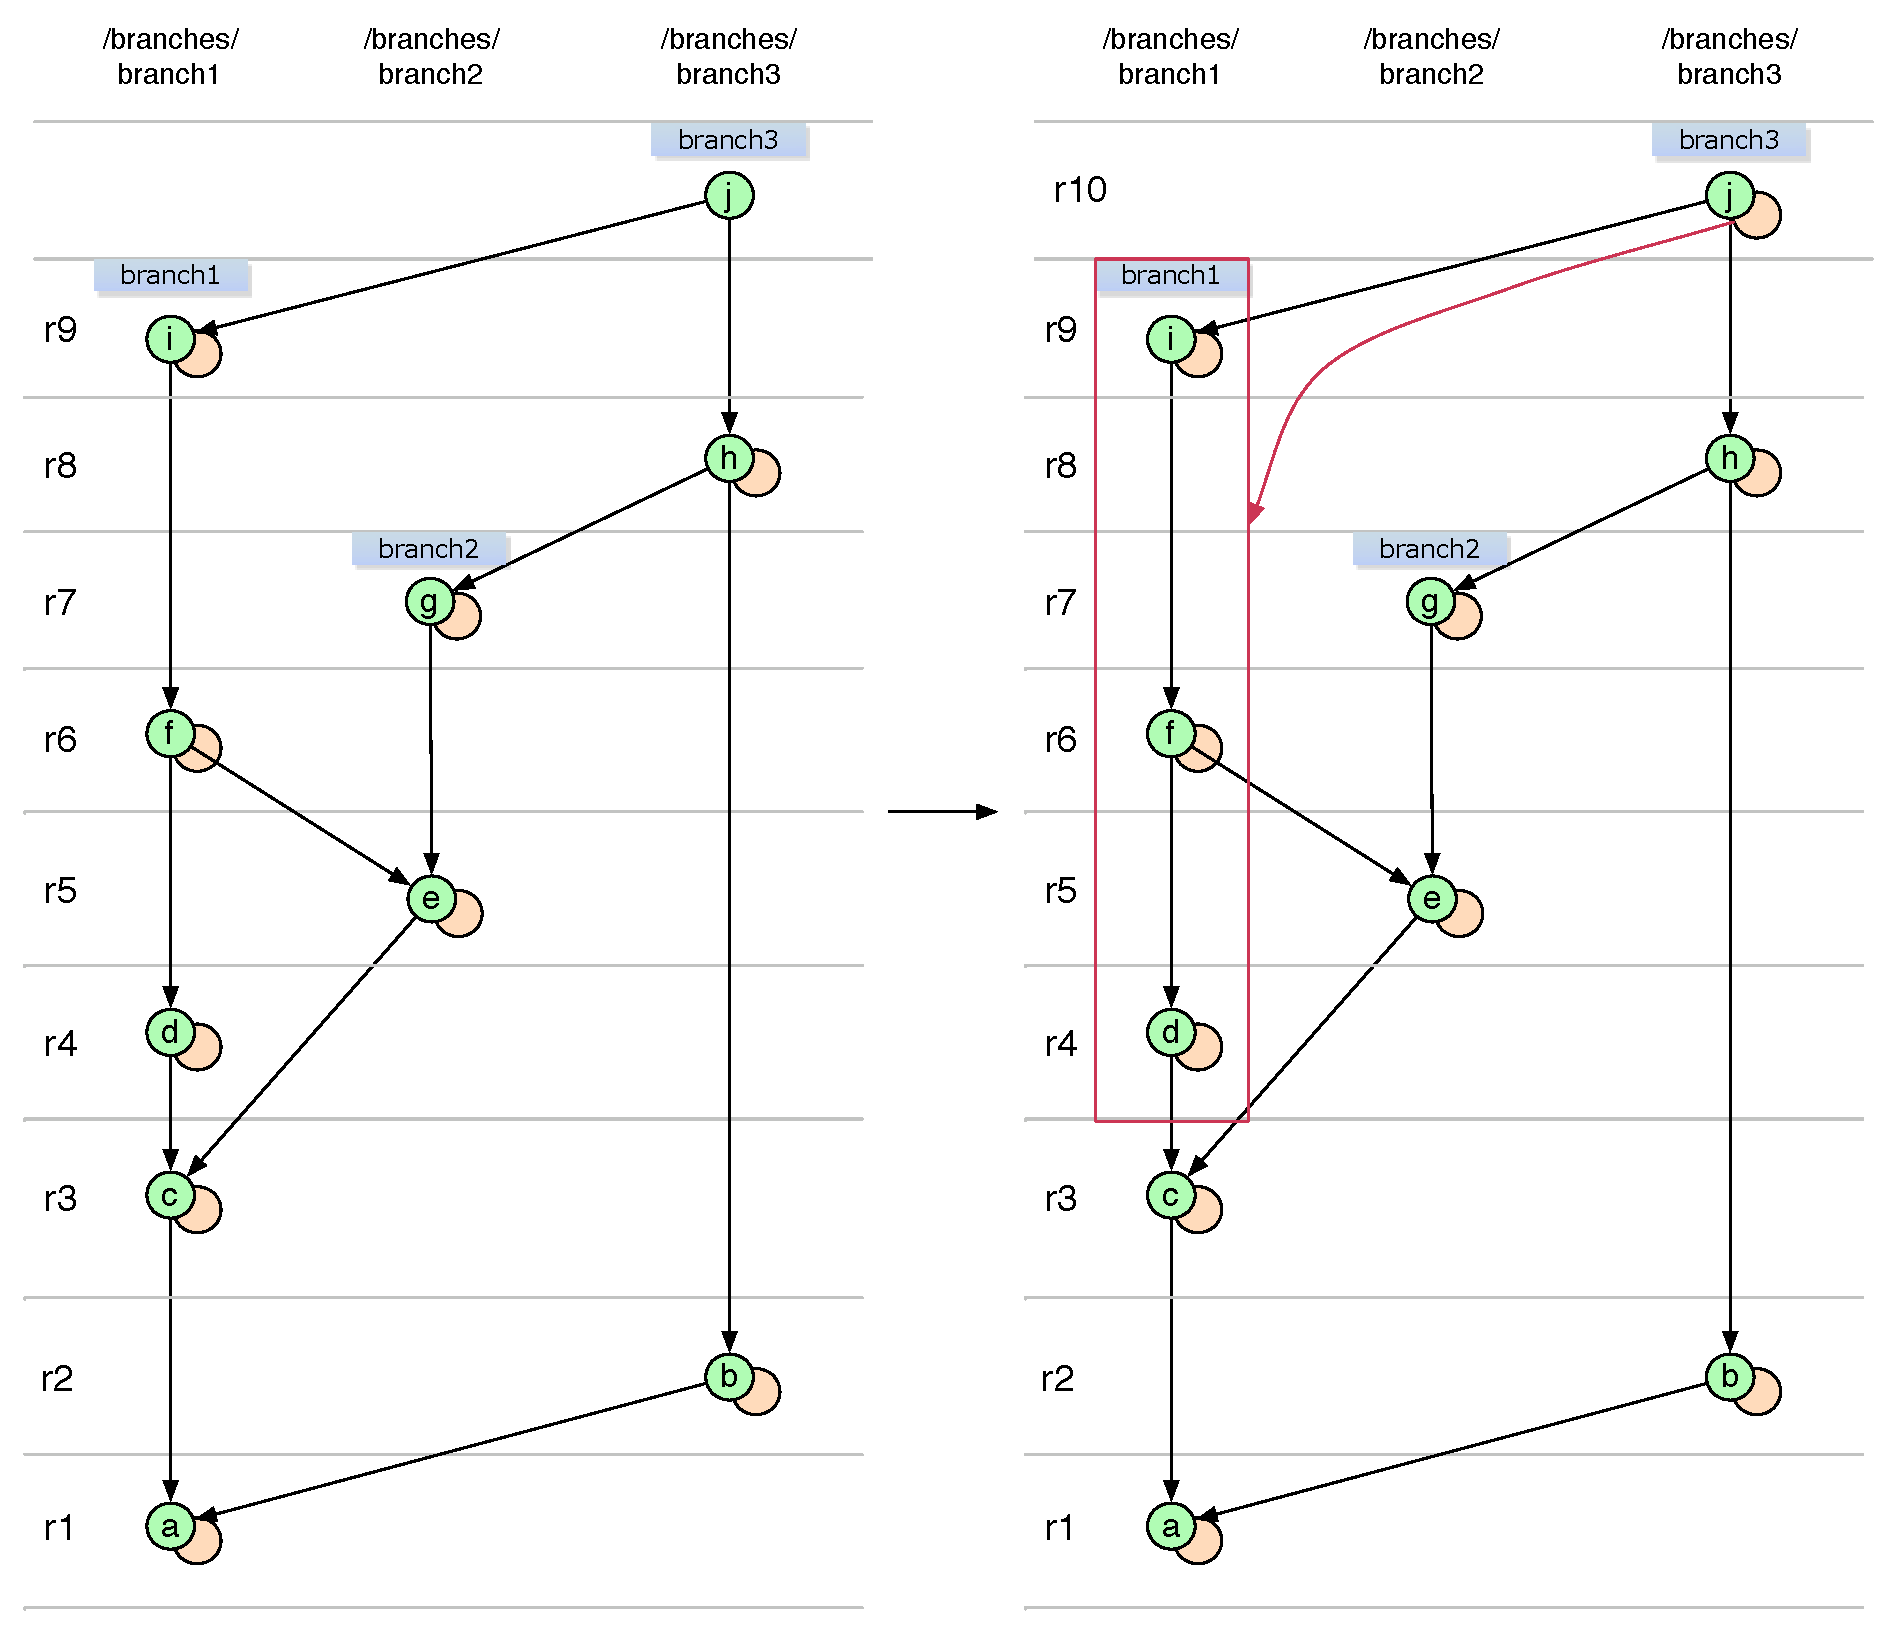
\includegraphics[width=\textwidth]{img/diagrams/merge_sequence_git_to_svn.pdf}%
\captionof{figure}{Merge of Git branch which is available from another branch being translated to a sequence of Subversion revisions.}
\label{merge_sequence_git_to_svn}%
\end{center}

The same holds in opposite direction: when Subversion user merged revisions corresponding to commits which appended to the branch close the history of the branch, Translator creates merge commit which represents this change. This scenario is depicted at diagram \ref{merge_sequence_svn_to_git}.

\begin{center}
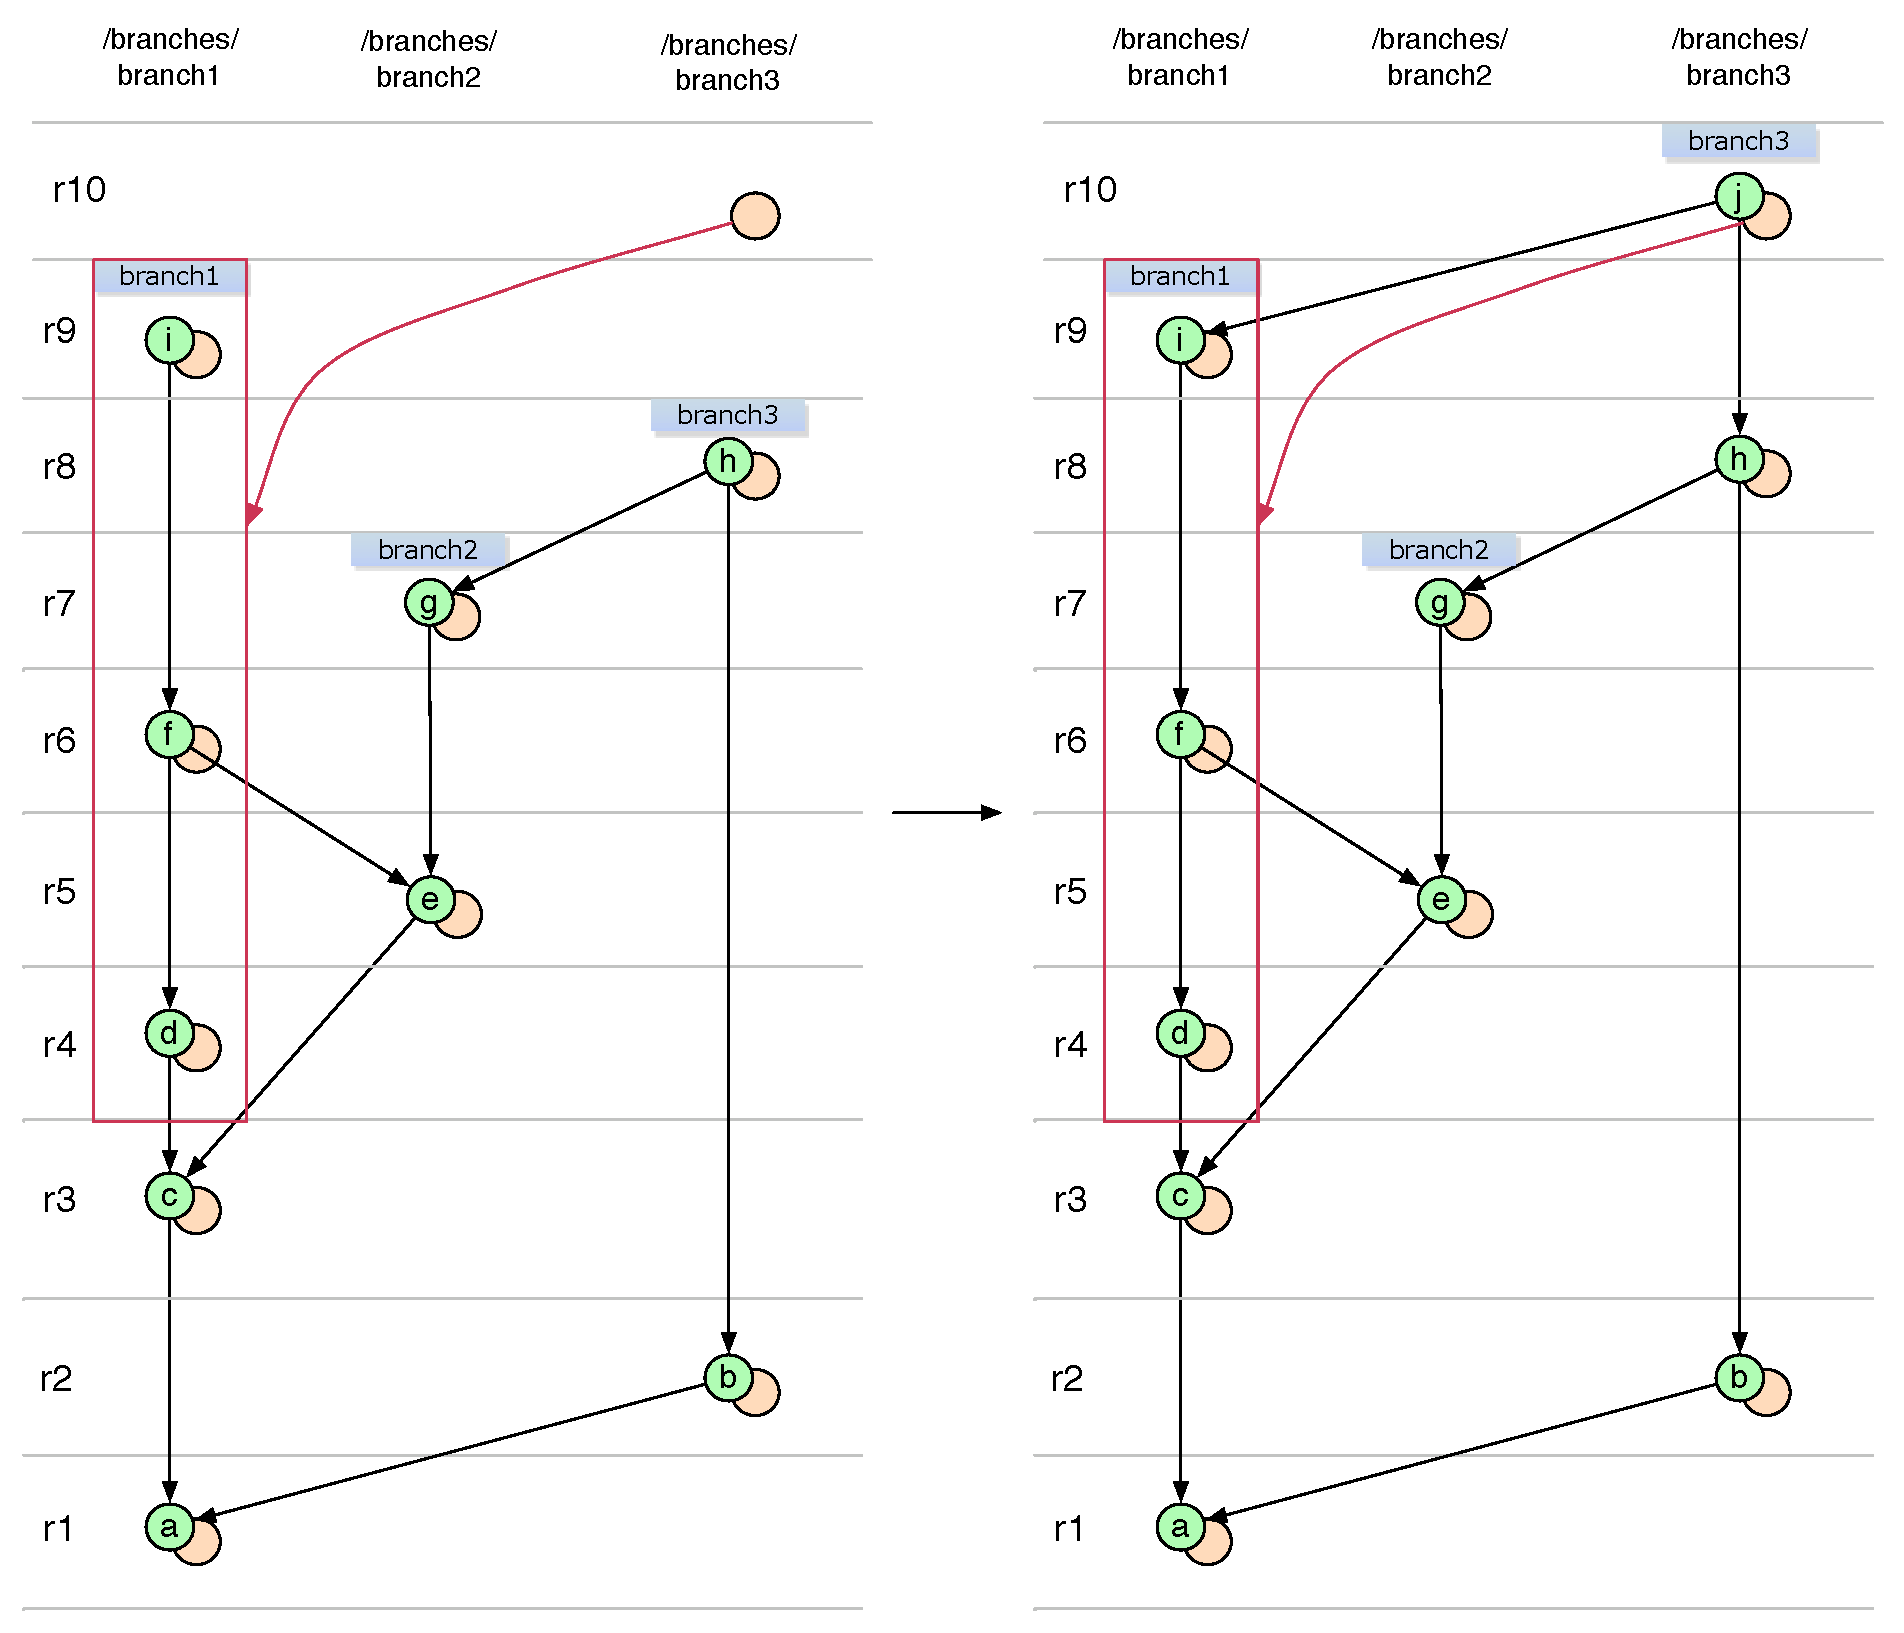
\includegraphics[width=\textwidth]{img/diagrams/merge_sequence_svn_to_git.pdf}%
\captionof{figure}{Merge of Git branch which is available from another branch being translated to a sequence of Subversion revisions.}
\label{merge_sequence_svn_to_git}%
\end{center}

Merged revisions may include only part of the history of a certain branch. 
This case might be a result of Subversion cherry-pick merges.
To translate this kind of merge, Translator merely creates regular Git commit with a single parent (see diagram \ref{no_merge_commit_cherry_pick_sequence_svn_to_git}). 

\begin{center}
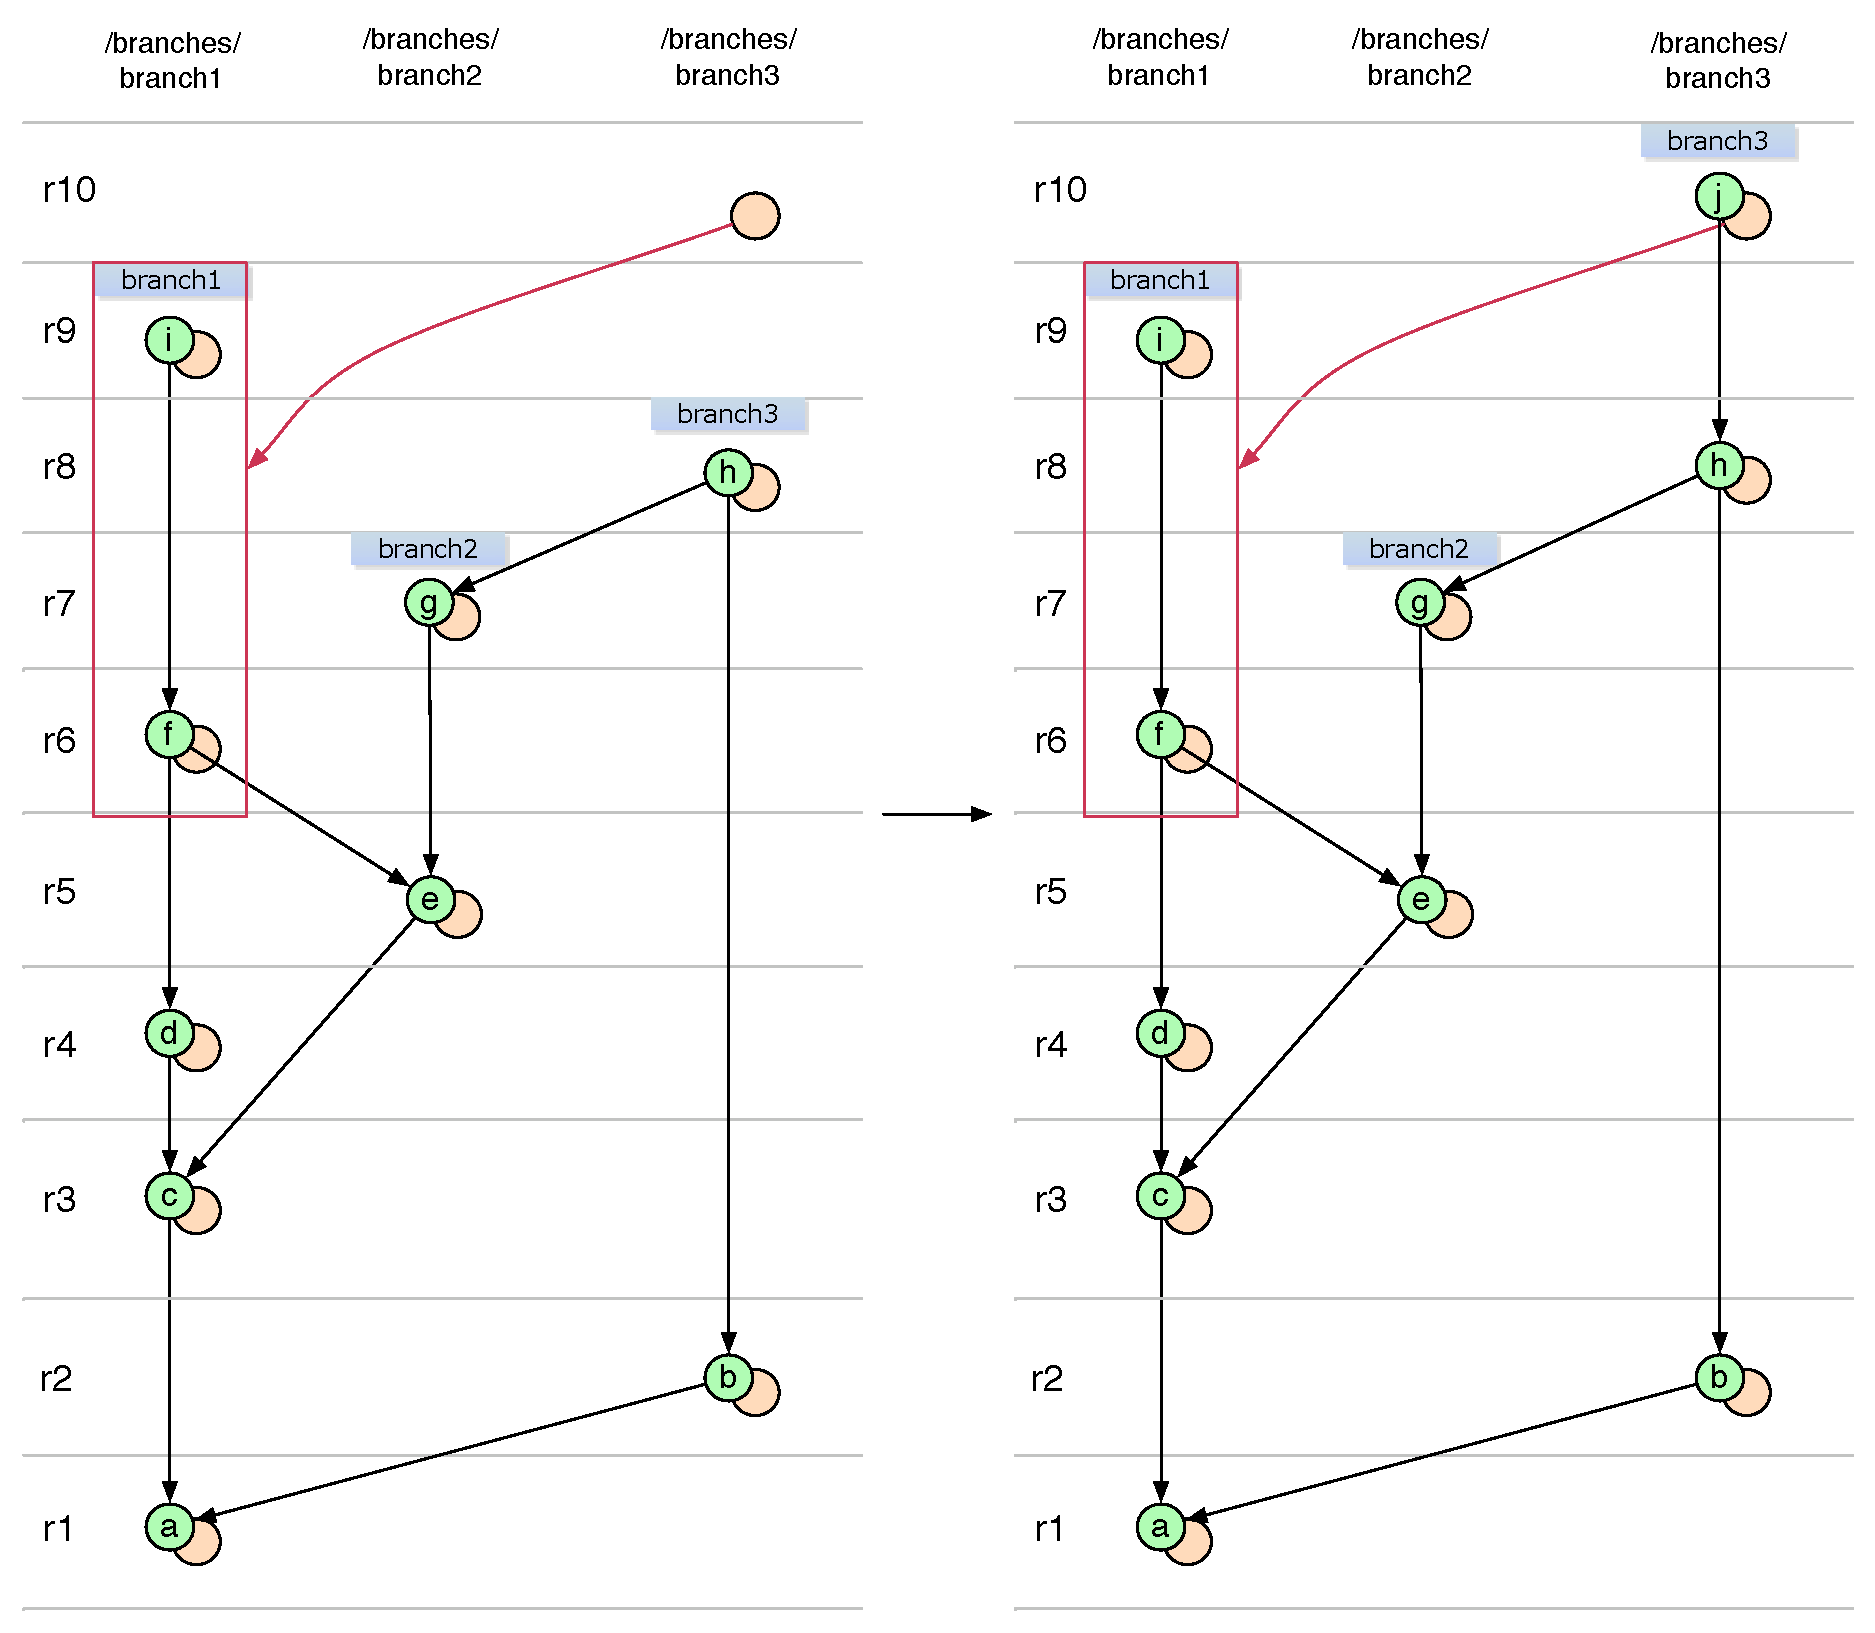
\includegraphics[width=\textwidth]{img/diagrams/no_merge_commit_cherry_pick_sequence_svn_to_git.pdf}%
\captionof{figure}{Merge of Git branch which is available from another branch being translated to a sequence of Subversion revisions.}
\label{no_merge_commit_cherry_pick_sequence_svn_to_git}%
\end{center}

\subsubsection{Octopus Merge}

Both Subversion and Git support so called \emph{octopus merge}, --- merge in which an arbitrary number of branches are merged into the target branch in a single revision or commit. 
\\\\
Translator supports this kind of merge in a way shown in the diagrams \ref{octopus_merge_git_to_svn} (for Git to Subversion translation) and \ref{octopus_merge_svn_to_git} (for Subversion to Git translation).

\begin{center}
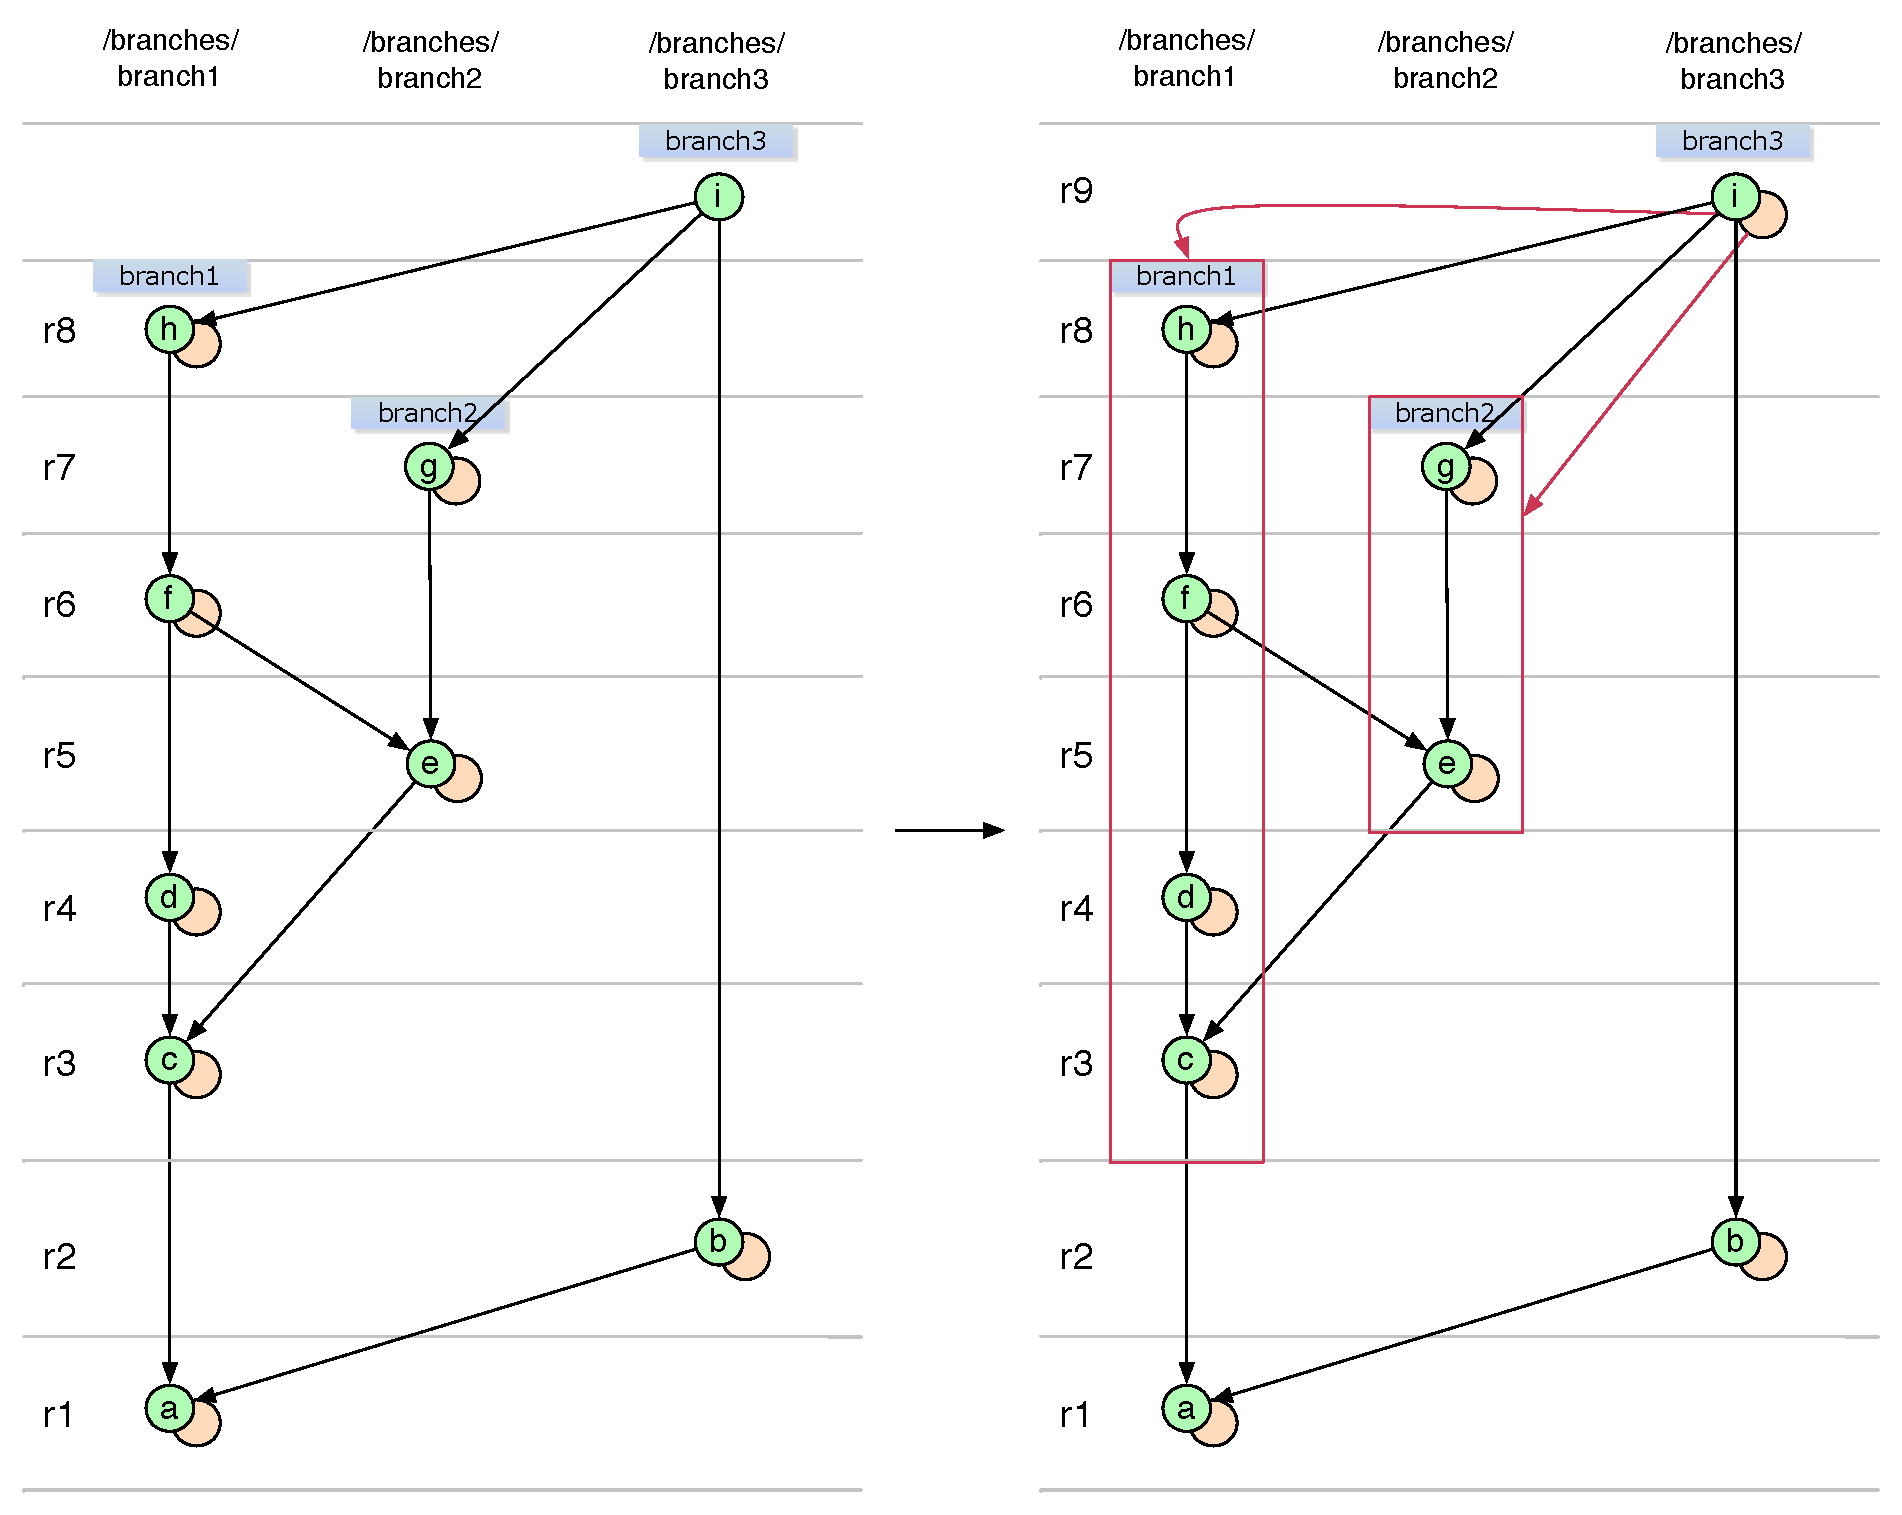
\includegraphics[width=\textwidth]{img/diagrams/octopus_merge_git_to_svn.pdf}%
\captionof{figure}{Octopus merge commit being translated to svn:mergeinfo change.}
\label{octopus_merge_git_to_svn}%
\end{center}

\begin{center}
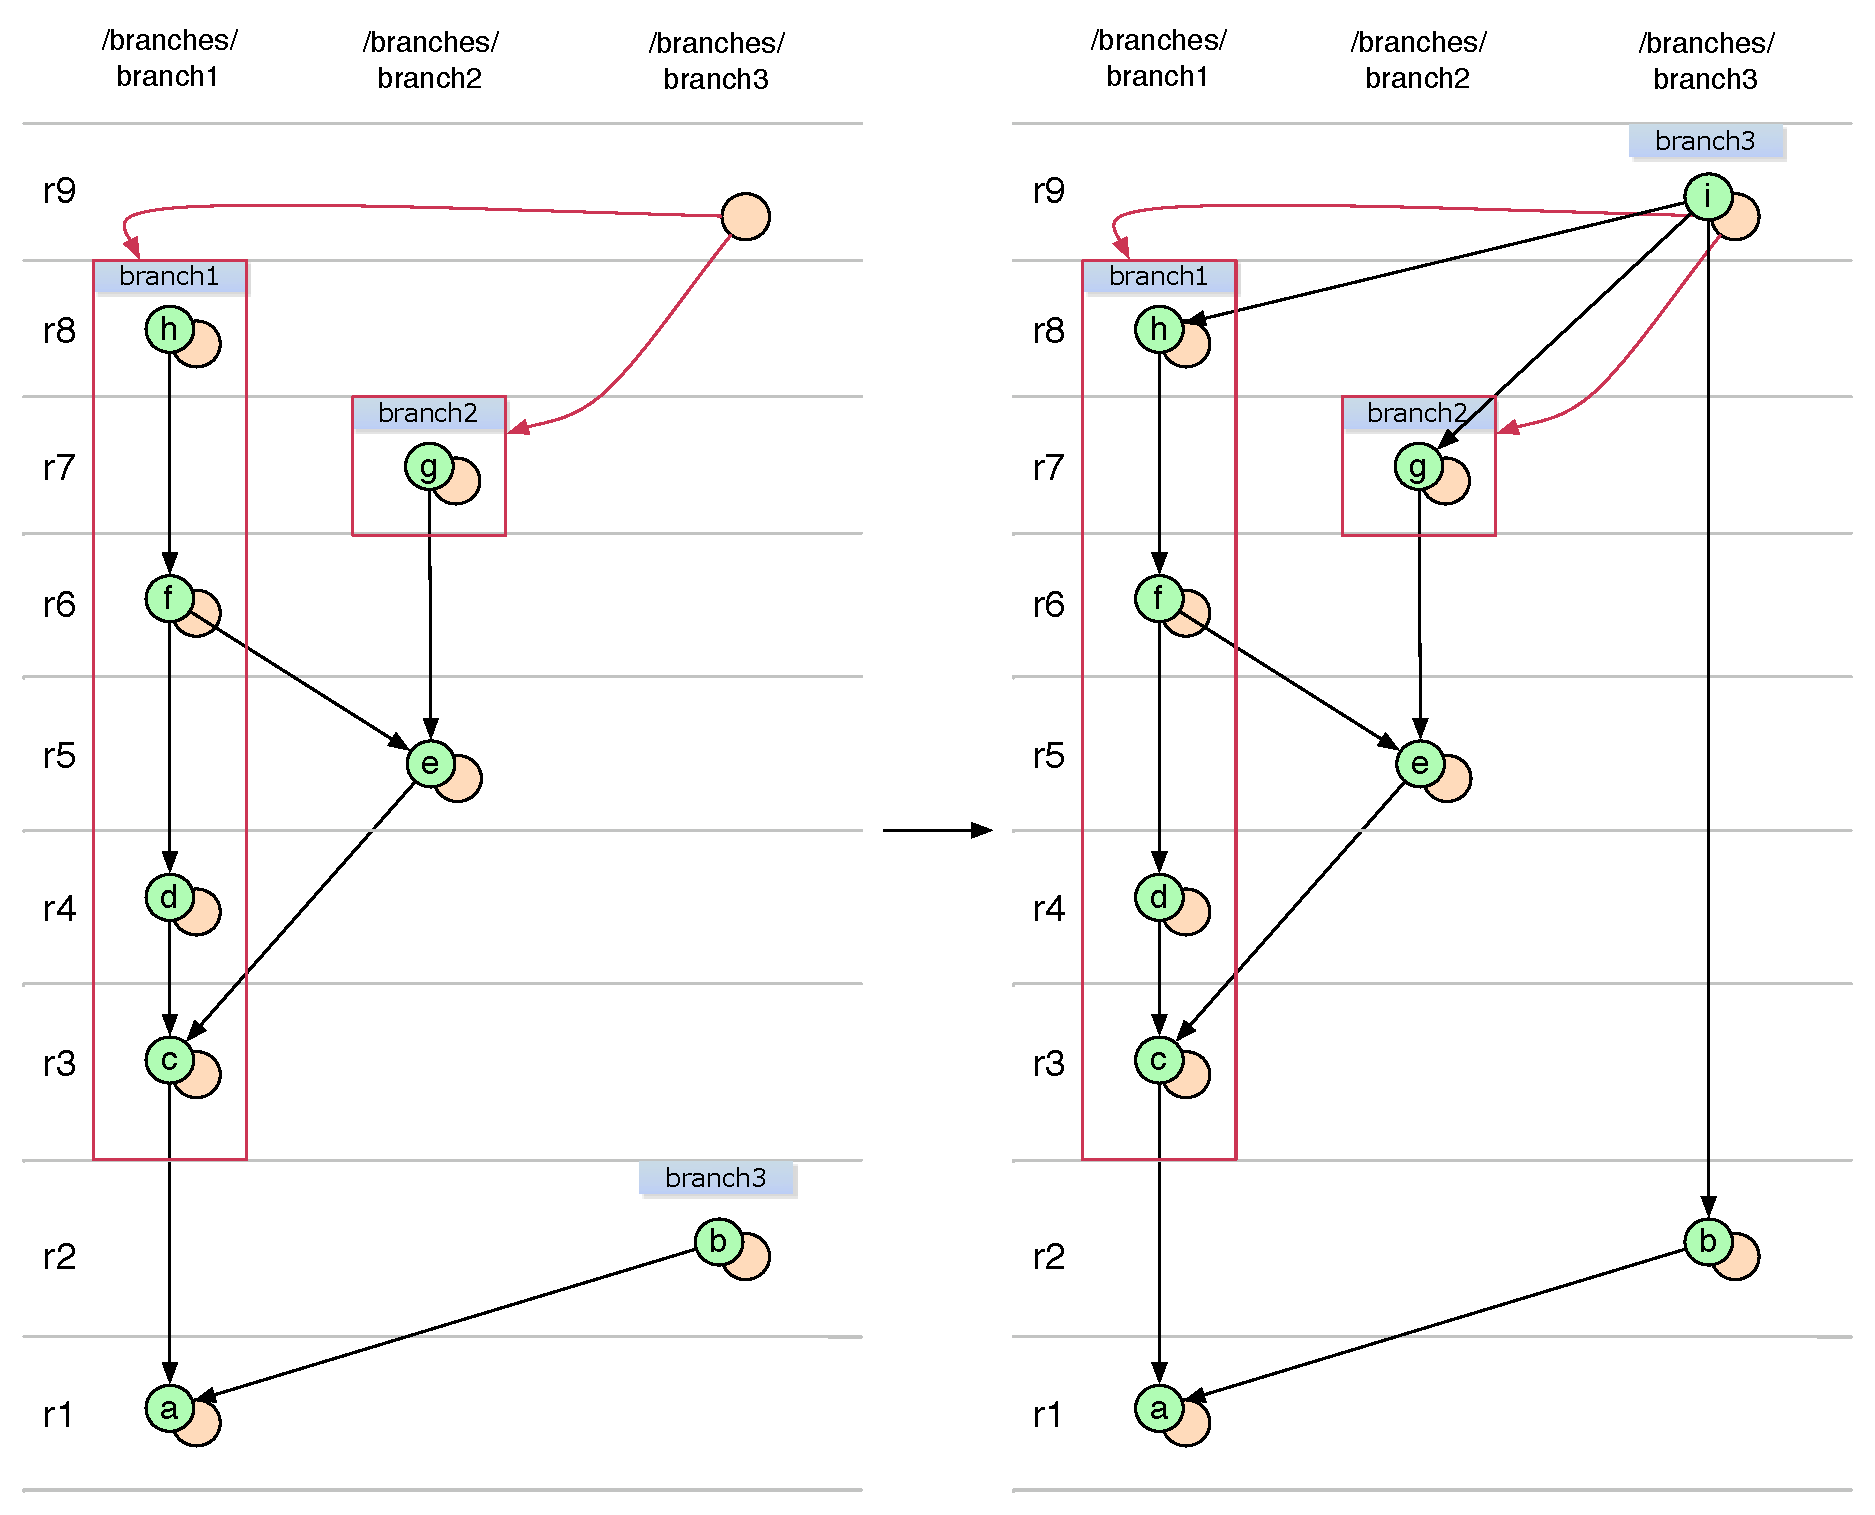
\includegraphics[width=\textwidth]{img/diagrams/octopus_merge_svn_to_git.pdf}%
\captionof{figure}{Change of svn:mergeinfo property being translated to octopus merge commit.}
\label{octopus_merge_svn_to_git}%
\end{center}
